%
\documentclass[11pt,a4paper]{article}

\usepackage{verbatim}
%% \usepackage{fancyhdr}
\usepackage{graphicx}
%% %\usepackage[leftmargin = 1in, rightmargin = 0.75in]{geometry}
%\usepackage{geometry}
%% \usepackage{latexsym}
\usepackage{amssymb}
\usepackage{amsmath}

\usepackage[hyperfootnotes=false]{hyperref}
\usepackage{subfig}
\usepackage{caption}
\usepackage{algpseudocode}
\usepackage{algorithm}
\usepackage{listings}

\usepackage{color}

\definecolor{dkgreen}{rgb}{0,0.6,0}
\definecolor{gray}{rgb}{0.5,0.5,0.5}
\definecolor{mauve}{rgb}{0.58,0,0.82}

\lstset{frame=tb,
  language=c++,
  morekeywords={occaKernel, __kernel, __global, occaConst, occaPointer, occaVariable, occaInnerId0, occaOuterId0, occaGlobalId0, occaOuterFor0, occaInnerFor0, occaKernelInfoArg, occaDims, occa, occa::device, occa::kernel, occa::memory, setup, malloc, setWorkingDims, buildKernelFromSource, free, copyFrom, copyTo},
  aboveskip=3mm,
  belowskip=3mm,
  showstringspaces=true,
  columns=flexible,
  basicstyle={\small\ttfamily},
  numbers=none,
  numberstyle=\tiny\color{gray},
  keywordstyle=\color{blue},
  commentstyle=\color{dkgreen},
  stringstyle=\color{orange},
  breaklines=true,
  breakatwhitespace=true,
  basicstyle=\small\normalfont\sffamily,    % the size of the fonts that are used for the code
  stepnumber=1,                % the step between two line-numbers. If it is 1 each line will be numbered
  numbersep=10pt,                         % how far the line-numbers are from the code
  tabsize=2,                              % tab size in blank spaces
  extendedchars=true,                     %
  breaklines=true,                        % sets automatic line breaking
  captionpos=t,                           % sets the caption-position to top
  mathescape=true,
  stringstyle=\color{white}\ttfamily, % Farbe der String
  showspaces=false,           % Leerzeichen anzeigen ?
  showtabs=false,             % Tabs anzeigen ?
  xleftmargin=17pt,
  framexleftmargin=17pt,
  framexrightmargin=17pt,
  framexbottommargin=5pt,
  framextopmargin=5pt,
  showstringspaces=false
}

\captionsetup[lstlisting]{format=listing,singlelinecheck=false, margin=0pt, font={sf}}

\newcommand{\pa}[2]{\frac{\partial #1}{\partial #2}}
\def\usFootnote{Department of Computational and Applied Mathematics, Rice University, 6100 Main Street - MS 134, Houston, TX 77005, USA}
\def\email{Corresponding author. \textit{Email addresses:
Rajesh.Gandham@rice.edu, timwar@rice.edu, fxgirald@nps.edu} }
\def\fxgFootnote{Department of Applied Mathematics, Naval Postgraduate School, 1 University Circle, Monterey, CA 93943}

\title{High performance discontinuous Galerkin methods for faster than real time tsunami simulations}
\author{R.~Gandham \footnote{\email} \textsuperscript{,}\footnote{\usFootnote},\
  T.~Warburton\footnotemark[\value{footnote}],\
  F.~X.~Giraldo\footnote{\fxgFootnote}}

\begin{document}

\maketitle
%% abstract
\begin{abstract}
%We describe the application of the high performance, high order discontinuous Galerkin methods for faster than real-time simulations of tsunami wave propagation. We adapt the methods described in \cite{gandham2014swe} and validate them with the tidal gauge recordings of 2004 Indian Ocean tsunami event. Our implementations use OCCA \cite{medina2014occa, occa2}, a portable and extensive multi-threading library.  OCCA\ library alleviates the need to completely re-design the solver to keep up with constantly evolving parallel programming models and hardware architectures. We present performance results for the real world tsunami simulations leveraging multiple different multi-threading APIs on GPU and CPU targets. 
Modeling the tsunami wave propagation is of great importance in developing warning systems and disastrous management planning. High fidelity models require very large scale computations. The requirement of running such simulations many times in stochastic analysis demands efficient and scalable simulators. In this paper, we consider two dimensional shallow water equations for modeling the tsunami wave phenomenon, a high order discontinuous Galerkin method   for the numerical simulation, and develop efficient algorithms that are tailored for SIMD architecture seen in modern GPUs. By adopting physically motivated multi-rate time stepping method and carefully designed implementations, we can simulate a realistic 10 hrs of 2004 Indian Ocean tsunami  in one minute on a single GPU workstation. We further demonstrate the efficiency of the developed simulator with 2011 Japan tsunami in global ocean. We use OCCA, an extensible multi-threading API that allows us to run the simulation on the many computing hardware architectures supporting any of CUDA, OpenCL, or OpenMP programming models.  


\end{abstract}


\section{Introduction}
\label{sec:intro}

$2004$ Indian Ocean tsunami, one of the deadliest tsunami in history, killed about $200,000$ people and cause a damage worth of billions of dollars, in $14$ countries in the Indian\ Ocean shorelines. Since then, there has been growing research and development in building tsunami warning systems around the world. These systems are designed to forecast tsunami arrivals and their impact in the coastal regions, hours before the waves arrive. 

 These forecasts involve simulating the wave propagation of tsunami waves over  large distances accurately in a timely manner, after a single or multiple earthquakes are detected in the ocean. This is challenging because of 
the complexity of the wave propagation due to the presence of largely varying length scales, varying bathymetry, and nonlinear effects near the shore. Stable, accurate and efficient algorithms are of great interest for these applications.

In this work, the two-dimensional shallow water equations are used to model the tsunami wave propagation. These equations are commonly accepted for modeling tsunami propagation \cite{george2006finite}. A high order discontinuous Galerkin (DG) discretization method on unstructure triangular meshes, is adapted for obtaining a numerical solution of the PDE. DG  methods are well suited for shallow water equations and wave propagation, in general, due to their good phase propagation properties, conservation properties, and capability of handling complex shoreline geometries. These methods achieve high order accuracy on irregular meshes by a high order polynomial representation of fluid properties in each element of the mesh. Nevertheless, these methods are computationally expensive compared to methods like finite volume, finite difference, and linear finite elements. However,  the recent advances in computing hardware architectures such as GPUs and many-core CPUs make it possible to achieve simulations in a reasonable time if the algorithms are well tuned to take advantage of the architecture trends. 

 To alleviate the need to write kernels for thread models like OpenMP, CUDA, and OpenCL separately, our implementations use extensive and unified many-core programming library called OCCA \cite{occa2}. This  gives us flexibility in choosing the most efficient multi-threading model for a given hardware architecture, without re-writing the code.
 
 This paper is organized as follows: In Section \ref{sec:governing}, the governing PDE model is introduced. In Section \ref{sec:discretization}, the discontinuous Galerkin space discretization and the multi-rate time stepping scheme are discussed briefly. In Section \ref{sec:datasets}, the data sets used for the simulation of Indian Ocean tsunami, the construction of initial conditions, boundary conditions, and implementation details of friction terms are elaborated. In Section \ref{sec:results}, the numerical validation results are presented along with the performance results. 

\section{Governing equations}
\label{sec:governing}
The shallow water equations are depth-integrated incompressible Navier-Stokes equations and are given in conservative form by,
\begin{eqnarray}
\label{eq:swe}
\pa{\eta}{t} + \pa{(hu)}{x} + \pa{(hv)}{y} &=& 0, \nonumber \\
\pa{}{t}(hu) + \pa{}{x}\left(hu^2 + \frac{1}{2}gh^2 \right) + \pa{}{y} (huv)&=& - gh\pa{B}{x} - \tau_{bx}, \nonumber \\
\pa{}{t}(hv) + \pa{}{x}(huv) + \pa{}{y}\left( hv^2 + \frac{1}{2}gh^2\right) &=&  -gh\pa{B}{y} - \tau_{by},
\end{eqnarray}
where, $\eta$ is free surface height above mean sea level, $h$ is the fluid column height, $u$, and $v$ are velocity components in longitudinal and latitudinal directions. $B$ is ocean bed topography or bathymetry, and $g$ is the acceleration due to gravity (see Fig. (\ref{fig:notation})  for the notation). $\tau_{bx}$ and $\tau_{by}$ are components of bottom friction force.
\begin{figure}[h!]
  \begin{center}
    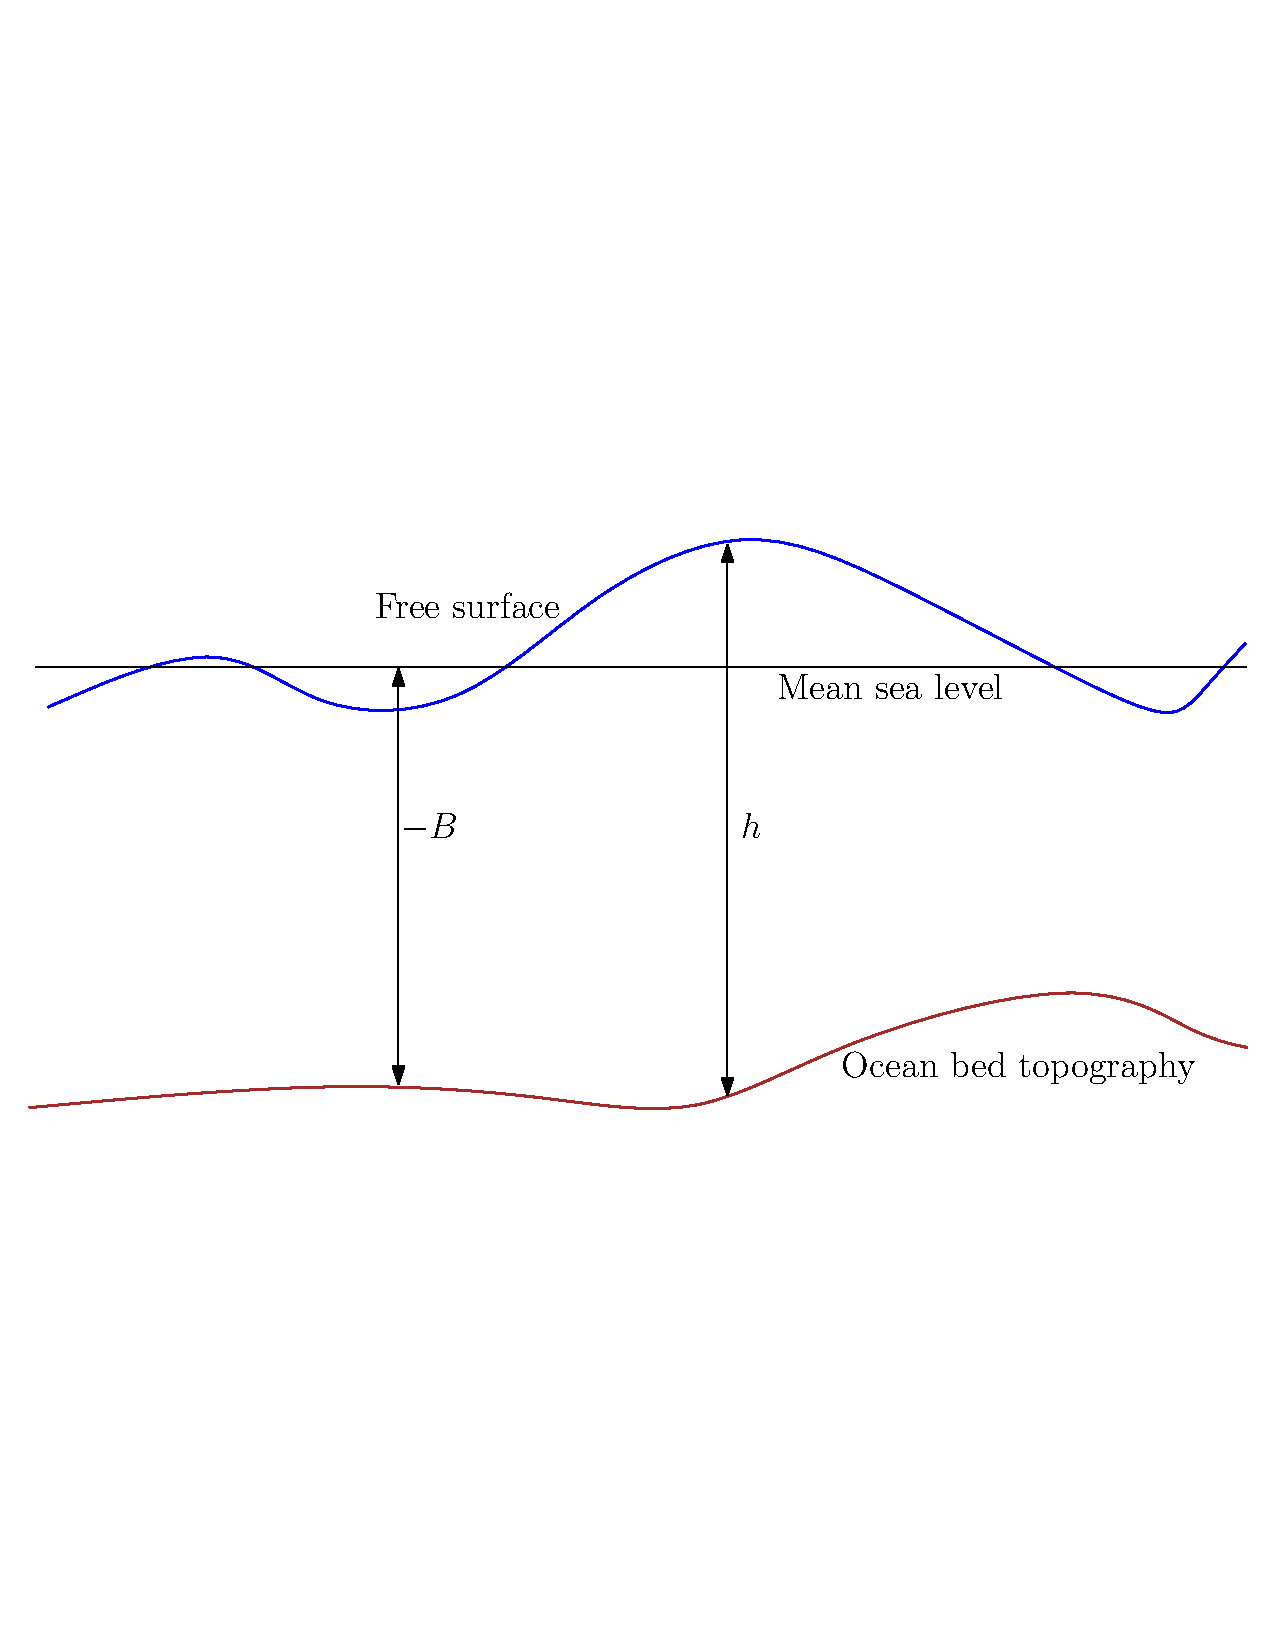
\includegraphics[trim=0cm 8cm 0cm 8cm,clip=true,width=0.5\linewidth]{./figures/bathymetry.pdf}
\caption{Diagram representation of notation of ocean domain.}
\label{fig:notation}
\end{center}
\end{figure}

\noindent In simplified form, these equations are represented as,
\begin{equation}
\label{eq:swe_conservative}
\pa{Q}{t} + \pa{F}{x} + \pa{G}{y} = S,
\end{equation}
here, $Q$ is the state vector, $F$, $G$ are the nonlinear flux vectors, and $S$ is the forcing vector. A high order discontinuous Galerkin method to obtain the solution of  Eq. (\ref{eq:swe_conservative}) and the details are discussed in the following  section.

\section{Numerical scheme}
\label{sec:discretization}
The computational domain   $\Omega \subset \mathbb{R}^2$, is partitioned into a set of non-overlapping, conforming triangles $\{ \Omega = \displaystyle\cup_{k} D^{k} \}$. The solution for $Q$ is approximated by $Q_H$, the components of which belong to the space of discontinuous piecewise polynomial of a given degree $N$ in each element ($P^{N}(D^{k})$). The PDEs in the Eq. (\ref{eq:swe_conservative}) are expressed in weak form. For each element, find $Q_H \in (P^{N}(D^{k}))^{3}$ such that for all $\phi \in P^{N}(D^{k})$ the below equation is true.
\begin{equation}
\left( \pa{Q_{H}}{t} , \phi \right)_{D^{k}} = \left( F, \pa{\phi}{x}\right)_{D^{k}} + \left( G, \pa{\phi}{y} \right)_{D^{k}} + (S, \phi)_{D^{k}} - \left(F^* n_x + G^* n_y,  \phi\right)_{\partial D^{k}}
\end{equation}
where $F^*$, $G^*$ are well-balanced Lax-Friedrich fluxes at the interface of each element \cite{xing2010positivity}. Here $(,)_{D^k}$ and $(,)_{\partial D^k}$ represent the inner products taken over the interior of the element $D^k$ and boundary of the element $D^k$, denoted by $\partial D^k$. Lagrange polynomials are used as a basis for the polynomial space in each element \cite{hesthaven2008nodal}, and the inner products are computed using numerical integration rules \cite{cools1999monomial}. The result is  a set of nonlinear ordinary differential equations with respect to time, $t$, given by,
\begin{equation}
\label{eq:ode}
\frac{d Q_{H}}{dt} = \mathcal{R}(Q_{H}) = \mathcal{N}(Q_{H}) + \mathcal{S}(Q_{H}^{g,+},Q_{H}^{g,-}),
\end{equation}

Here, $\mathcal{R}$  is the spatial discretization operator and $\mathcal{N}$, $\mathcal{S}$ are the nonlinear operators corresponding to interior (or volume) and interface (or surface) integrations. $Q_{H}^{g}$ is a vector of  the state variables at the Gauss quadrature nodes at the interface of each element. $Q_{H} ^{g,+}$ and $Q_{H}^{g,-}$ represent the positive and negative traces of the solution at the element interfaces. The ODEs  in  Eq. (\ref{eq:ode}) are integrated using a multi-rate $3^{rd}$ order Adams-Bashforth time stepping method to obtain the solution at a given time $t$.

Typically, the meshes used for these simulations have largely varying mesh length scales to be able to capture the effects of varying bathymetry. For a global scheme, the overall time step size is determined by the smallest mesh length scale so that the numerical scheme is stable. Whereas, a multi-rate scheme allows the elements to be integrated using the local characteristic length scales in the mesh. This is done efficiently by grouping the elements into levels based on their characteristic lengths and integrating the elements in a level with a fixed time step size. After mesh generation, the individual time step for each element is evaluated and elements with an allowable time step $\Delta t$ are grouped into a level $l$ if $2^{l-1} \Delta t _{min} \le \Delta t < 2^l \Delta t _{min}$. All elements in level $l$ are integrated with a time step $2^{l-1} \Delta t_{min}$. Once the elements are grouped into levels, they are re-grouped such that any two neighbor elements are at most one level apart. The elements with smallest allowable time step size (or finer elements) are integrated first, followed by elements with larger allowable time step size (or coarser elements). At the interface of the coarse and fine elements, the field values of the coarse elements at intermediate time step are obtained using the extrapolation of the AB time stepping scheme. The algorithm for multi-rate scheme is described in detail in \cite{gandham2014swe}. 

The resulting scheme does not guarantee that the fluid column height is positive during the simulation. A post-processing step (or positivity preserving limiter) is performed to ensure the positivity of the fluid height after every time step at each level. In this method, the numerical solution for the fluid height and momentum in a partially dry/wet element is restricted to a linear polynomial. The slope of the restricted polynomial for the fluid height is modified such that the minimum fluid height is above a chosen cutoff value. This method ensures the conservation of mean for fluid height and momentum. For completely dry elements, the fluid height is set to be the chosen cutoff value.

\section{Case studies}
The main purpose of developing efficient numerical method is to model real
world tsunami events and obtain accurate predictions in a timely manner. To demonstrate the applicability of the developed method, we consider two case studies. One is 2004 Indian Ocean tsunami caused by earthquakes in Sumatra island and the other is 2011 Japan tsunami caused by an earthquake in the coast of Tohuku. 

In order to model these events, it is important to obtain  accurate coastal
data, bathymetry distribution for the domain of interest, constructing the initial conditions for the forward wave modeling and setting up the boundary conditions. These are described in here.   
%\subsection{Case I: Indian Ocean tsunami modeling}
\label{sec:datasets}
 
\subsection{Coastal data}
Coastal data sets are needed to define the computational domain for these simulations. These are obtained from the Global Self-consistent, Hierarchical, High-resolution Shoreline (GSSHG  \cite{wessel2013gshhg}) a database provided by National Oceanographic and Atmospheric Administration (NOAA). 

\subsection{Computational mesh}
Triangular mesh aligned with complex coastlines is generated with an open-source mesh generation software tool GMSH. For the simulation in Indian Ocean, the mesh on the spherical surface is obtained from GMSH and is projected on 2D plane using a Mercator projection scheme. The generated mesh is shown in Fig (\ref{fig:indian_ocean_mesh}). This triangular mesh was provided to us by  the Alfred Wegner Institute, Germany.
For the simulation on world ocean, the mesh on the stereographic plane is obtained and projected on to the spherical surface. The generated mesh is show in Fig(\ref{fig:world_ocean_mesh}). This triangular mesh was provided to us by Bruno Seny. 
\begin{figure}[h!]
\begin{center}
\centering
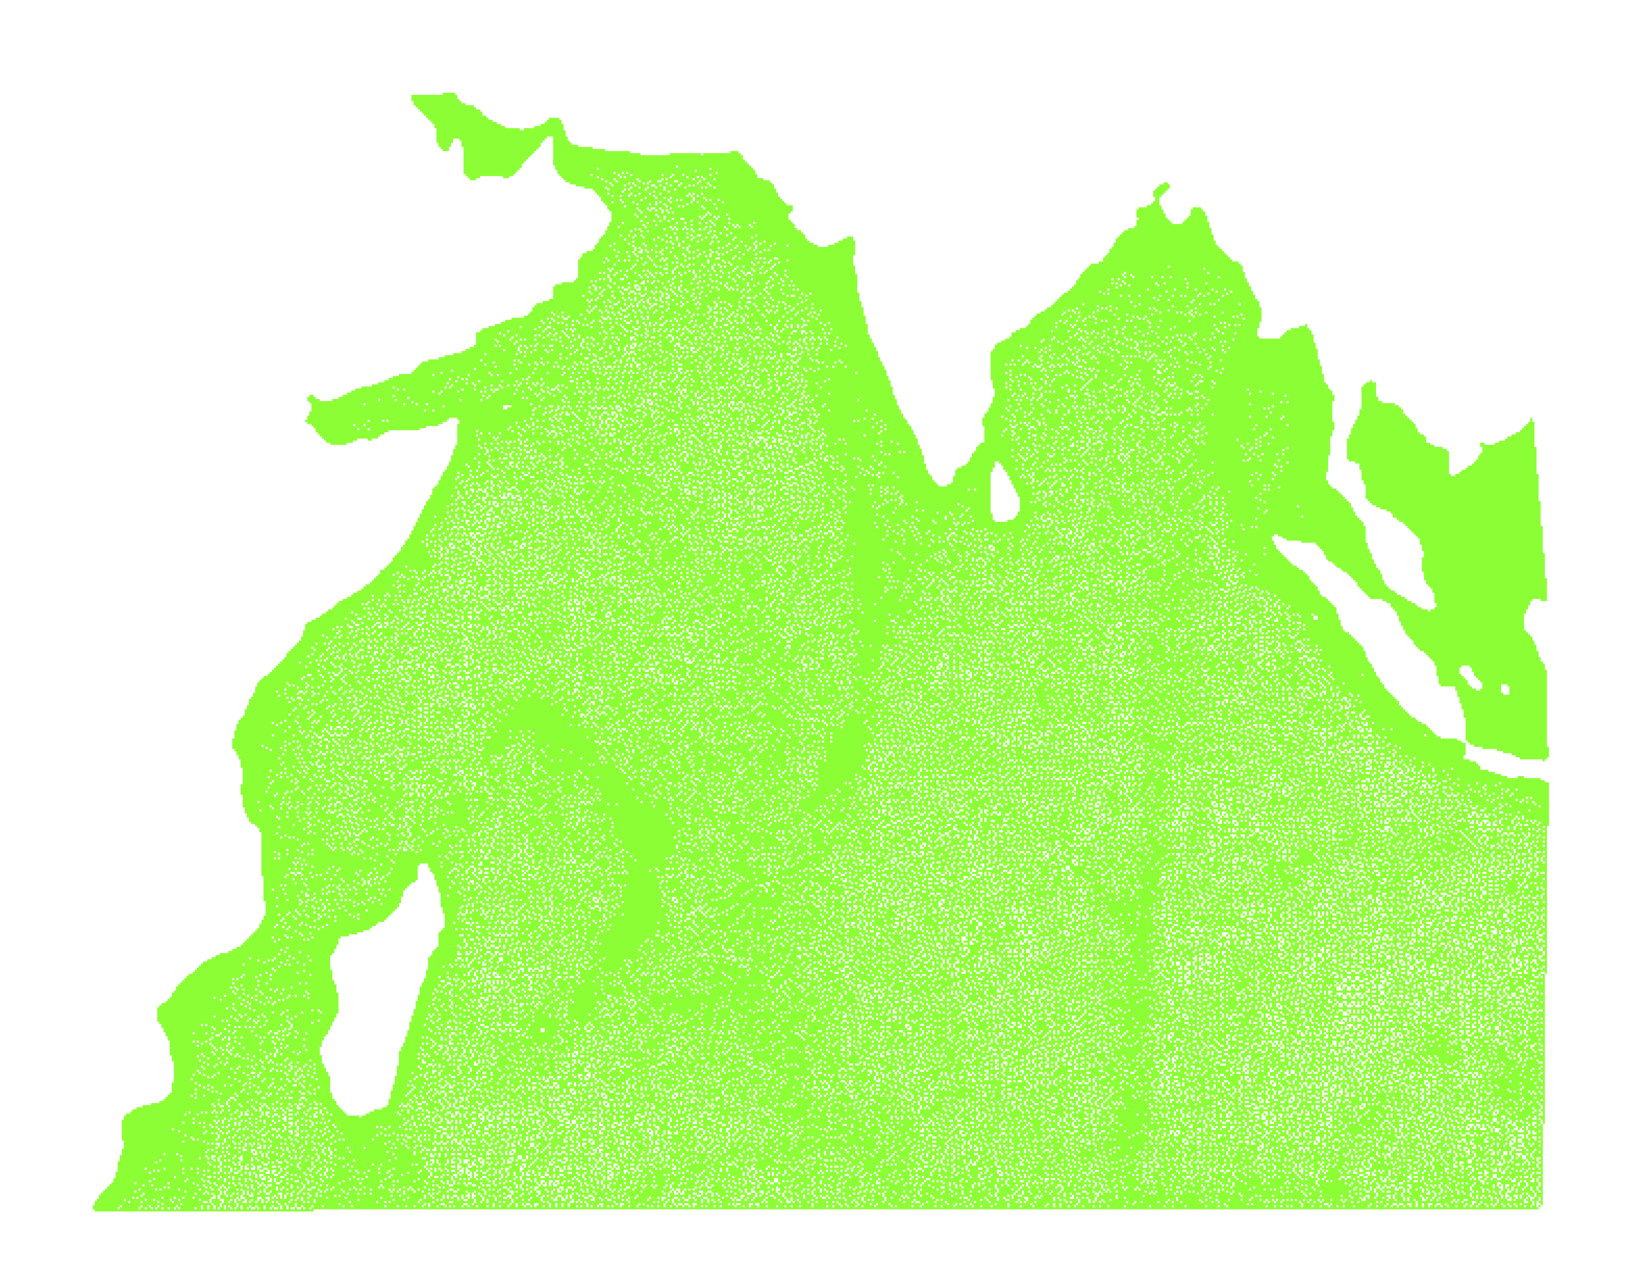
\includegraphics[trim=1.5cm 1cm 1.5cm 1.5cm,clip=true,width=0.5\linewidth]{./figures/IndianOcean.pdf}
\caption{\emph{Coastal aligned triangulation with 130,000 triangles of Indian Ocean.  Mesh and bathymetry distribution are provided by the Alfred Wegner Institute, Germany.}}
\label{fig:indian_ocean_mesh}
\end{center}
\end{figure}

\begin{figure}[h!]
\begin{center}
\centering
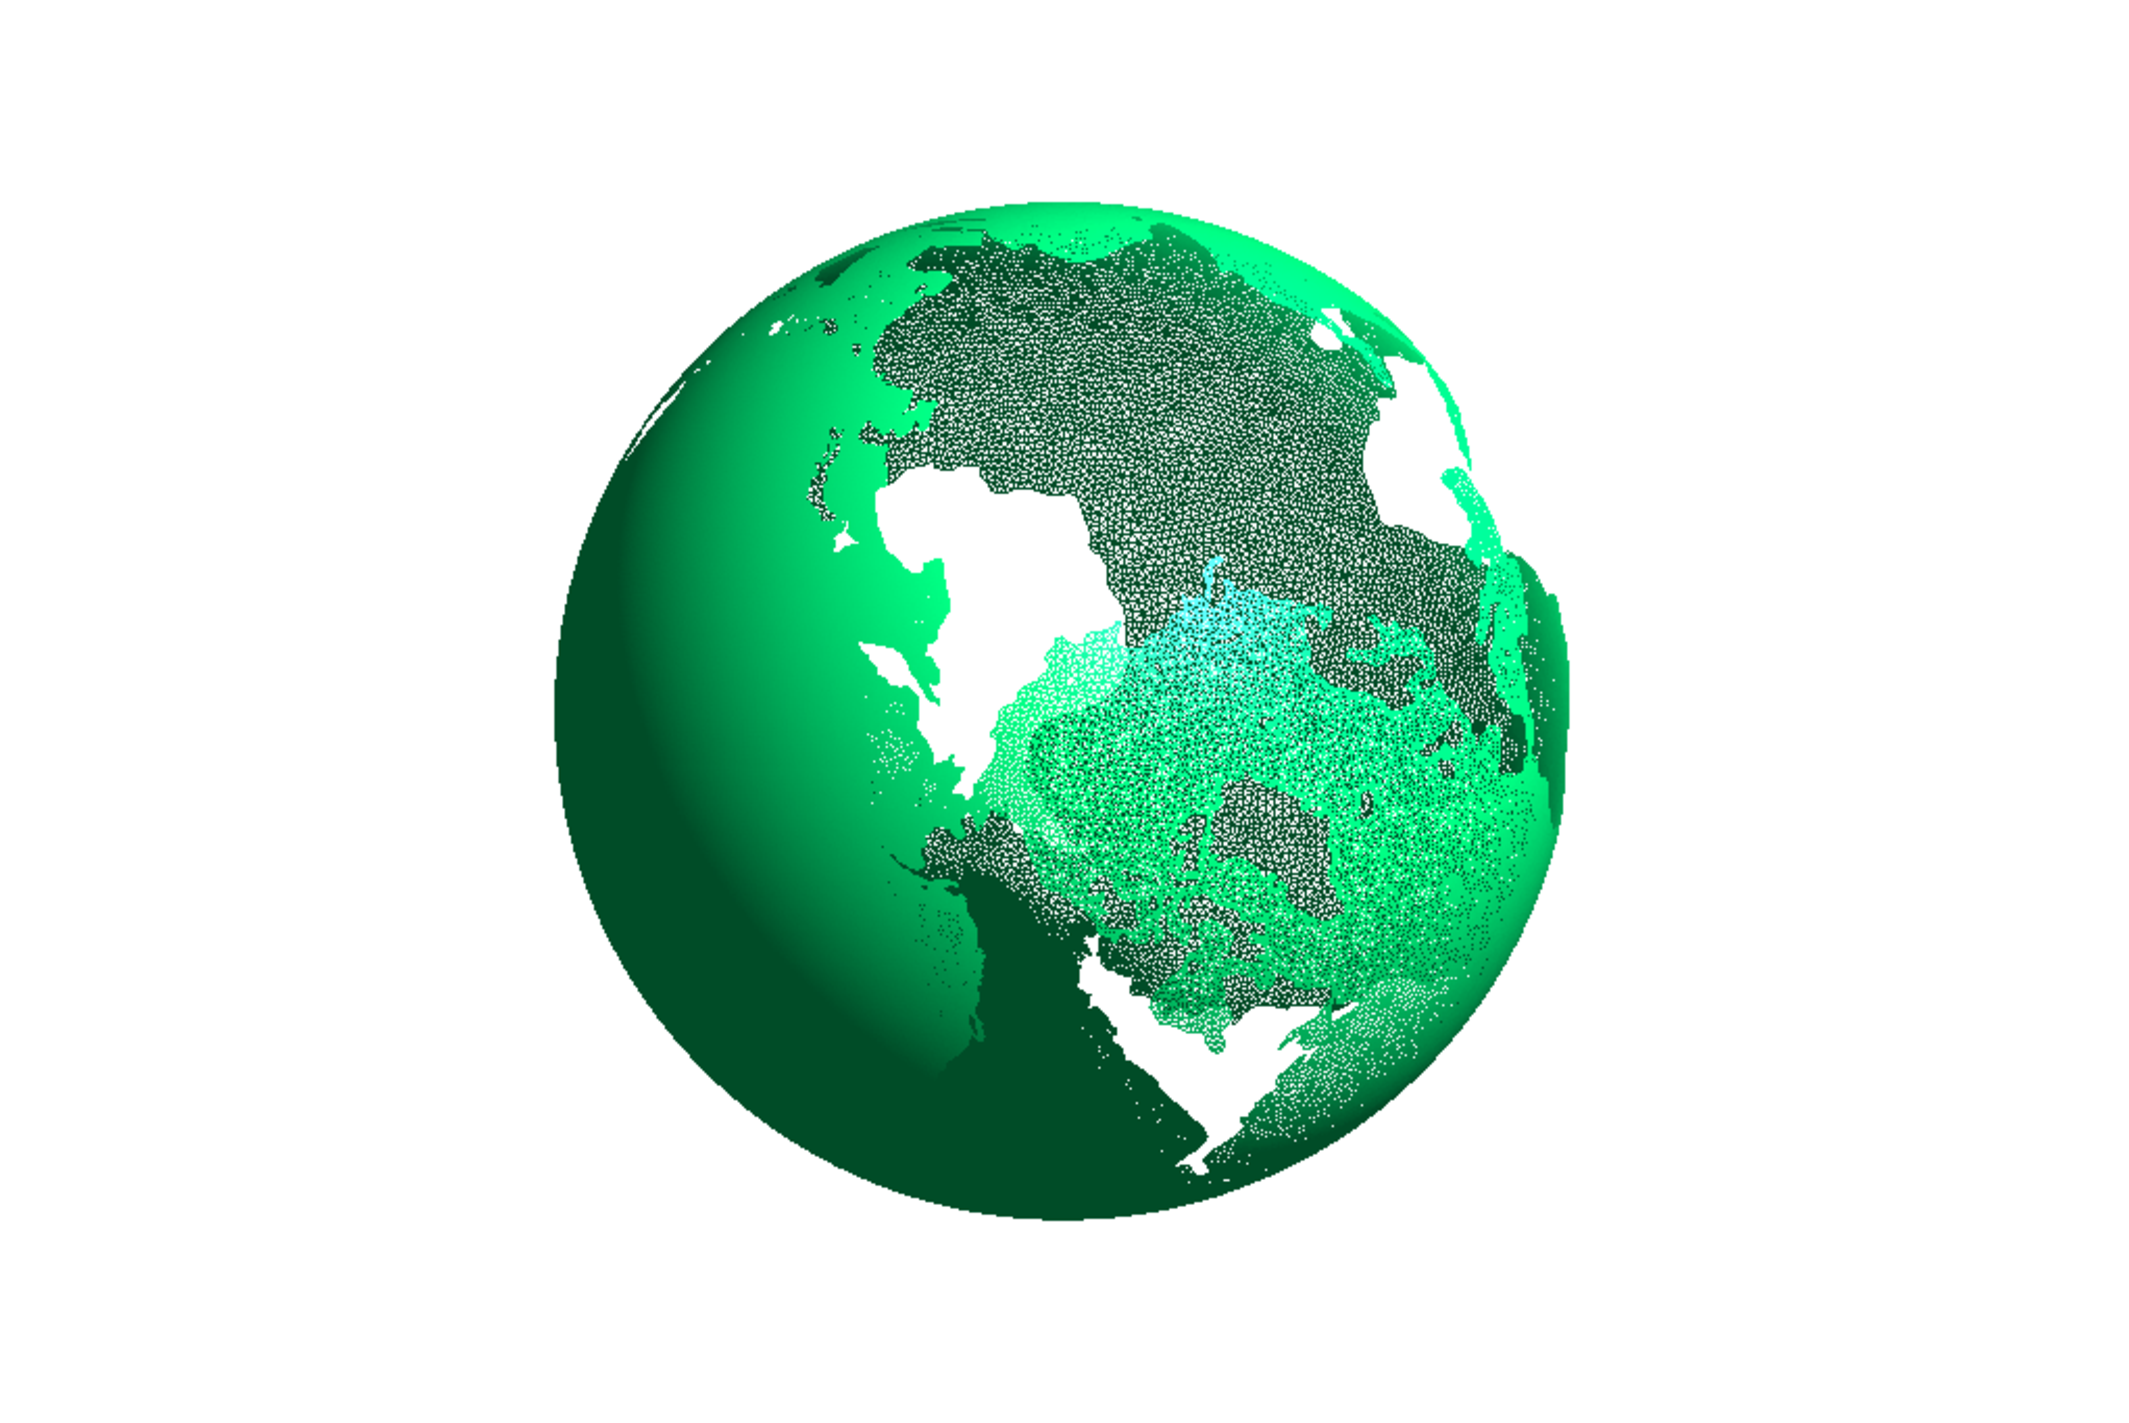
\includegraphics[trim=9cm 3cm 9cm 3cm,clip=true,width=0.5\linewidth]{./figures/globalOceanSphere.pdf}
\caption{\emph{Coastal aligned triangulation with 1,757,467 triangles of global
Ocean.}}
\label{fig:world_ocean_mesh}
\end{center}
\end{figure}

\subsection{Bathymetry distribution}
Accurate information on the ocean bed topography (or bathymetry) is crucial for tsunami simulations. This is because the speed of the tsunami waves is dictated by the water column height. Here, the ETOPO  \cite{amante2009etopo1} dataset from NOAA is used for the distribution of bathymetry. This information is also incorporated into mesh generation for defining mesh length scales.  The distribution of bathymetry in the Indian Ocean is shown in Fig (\ref{fig:indian_ocean_bathy}), in the world ocean is shown in Fig (\ref{fig:world_ocean_bathy}).
\begin{figure}[h!]
\begin{center}
\centering
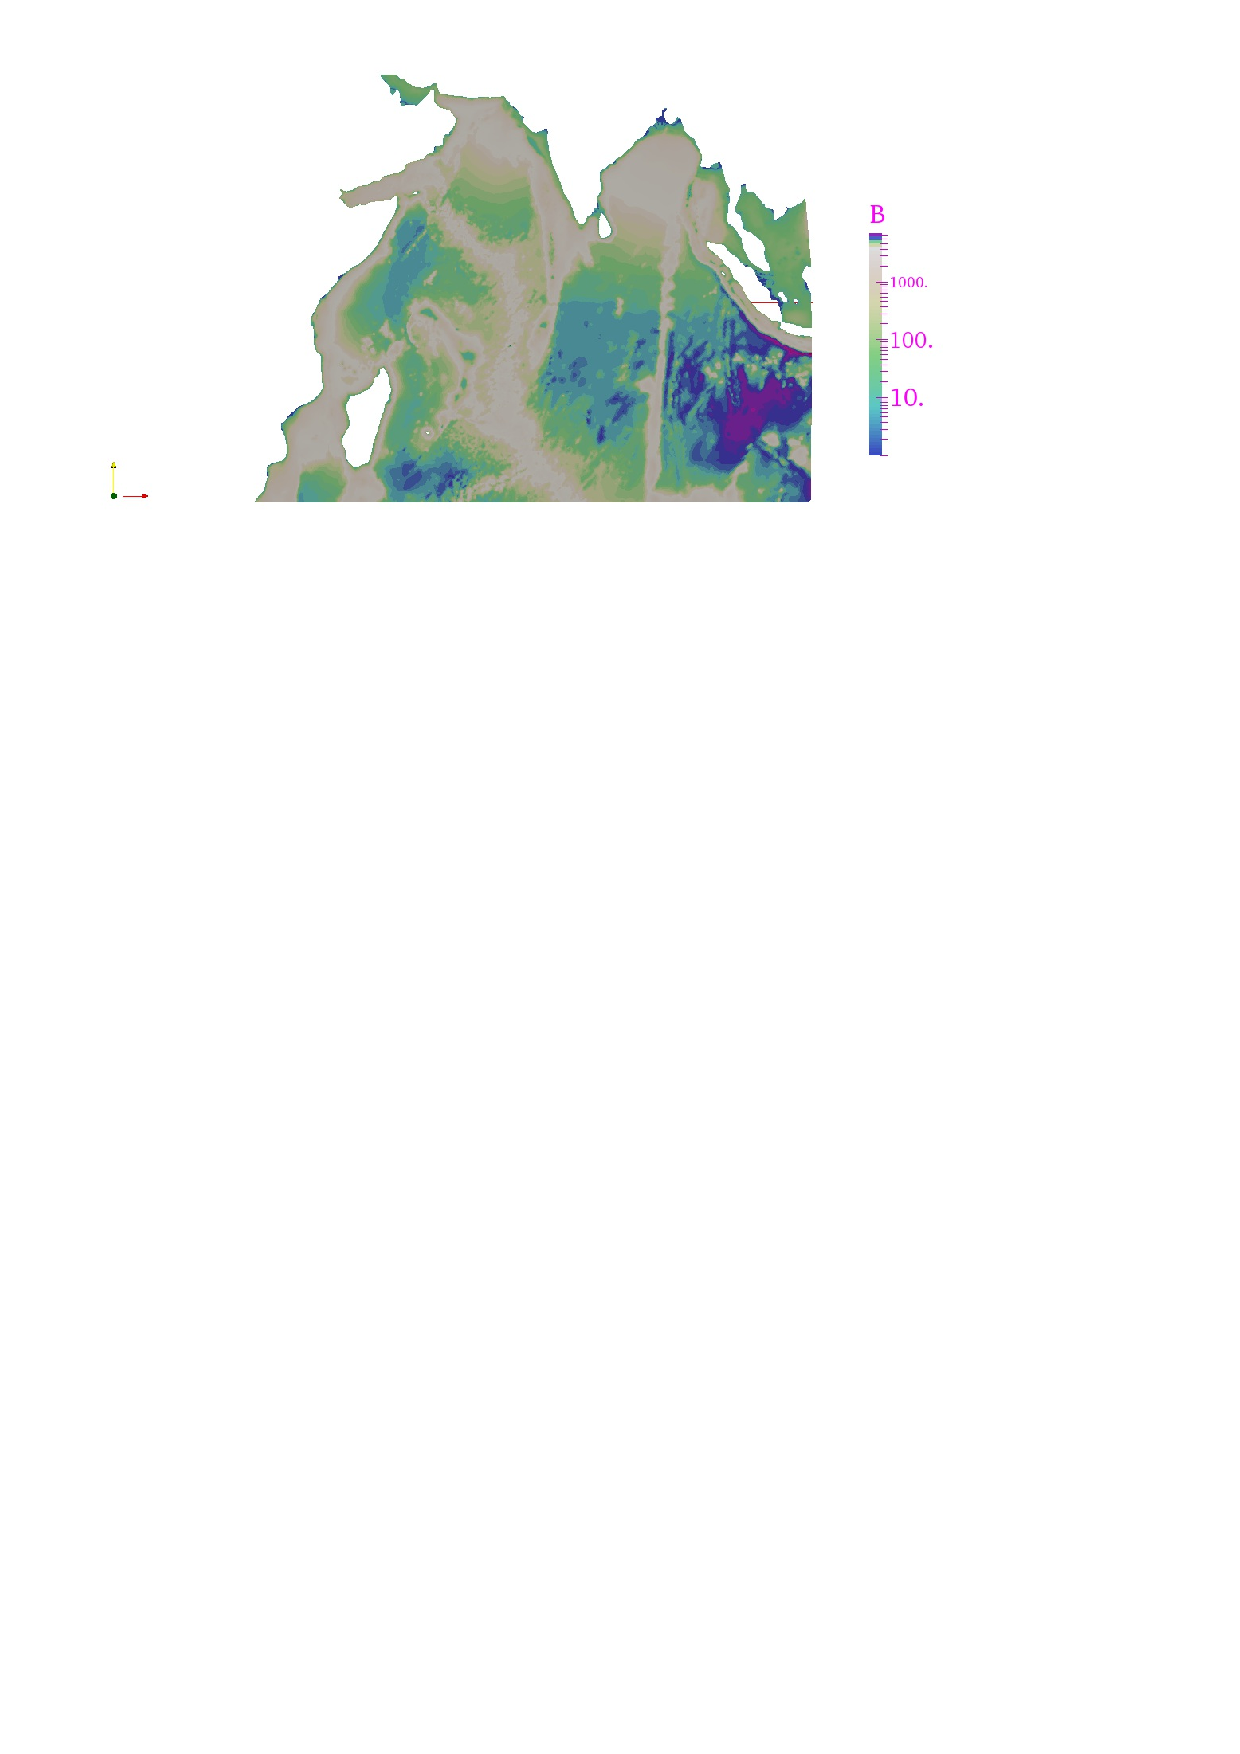
\includegraphics[trim=4.3cm 21.25cm 5.25cm 1.25cm,clip=true,width=0.5\linewidth]{./figures/IndianOceanBathy.pdf}
\caption{\emph{Bathymetry distribution (in meters) in Indian Ocean.}}
\label{fig:indian_ocean_bathy}
\end{center}
\end{figure}
\begin{figure}[h!]
\begin{center}
\centering
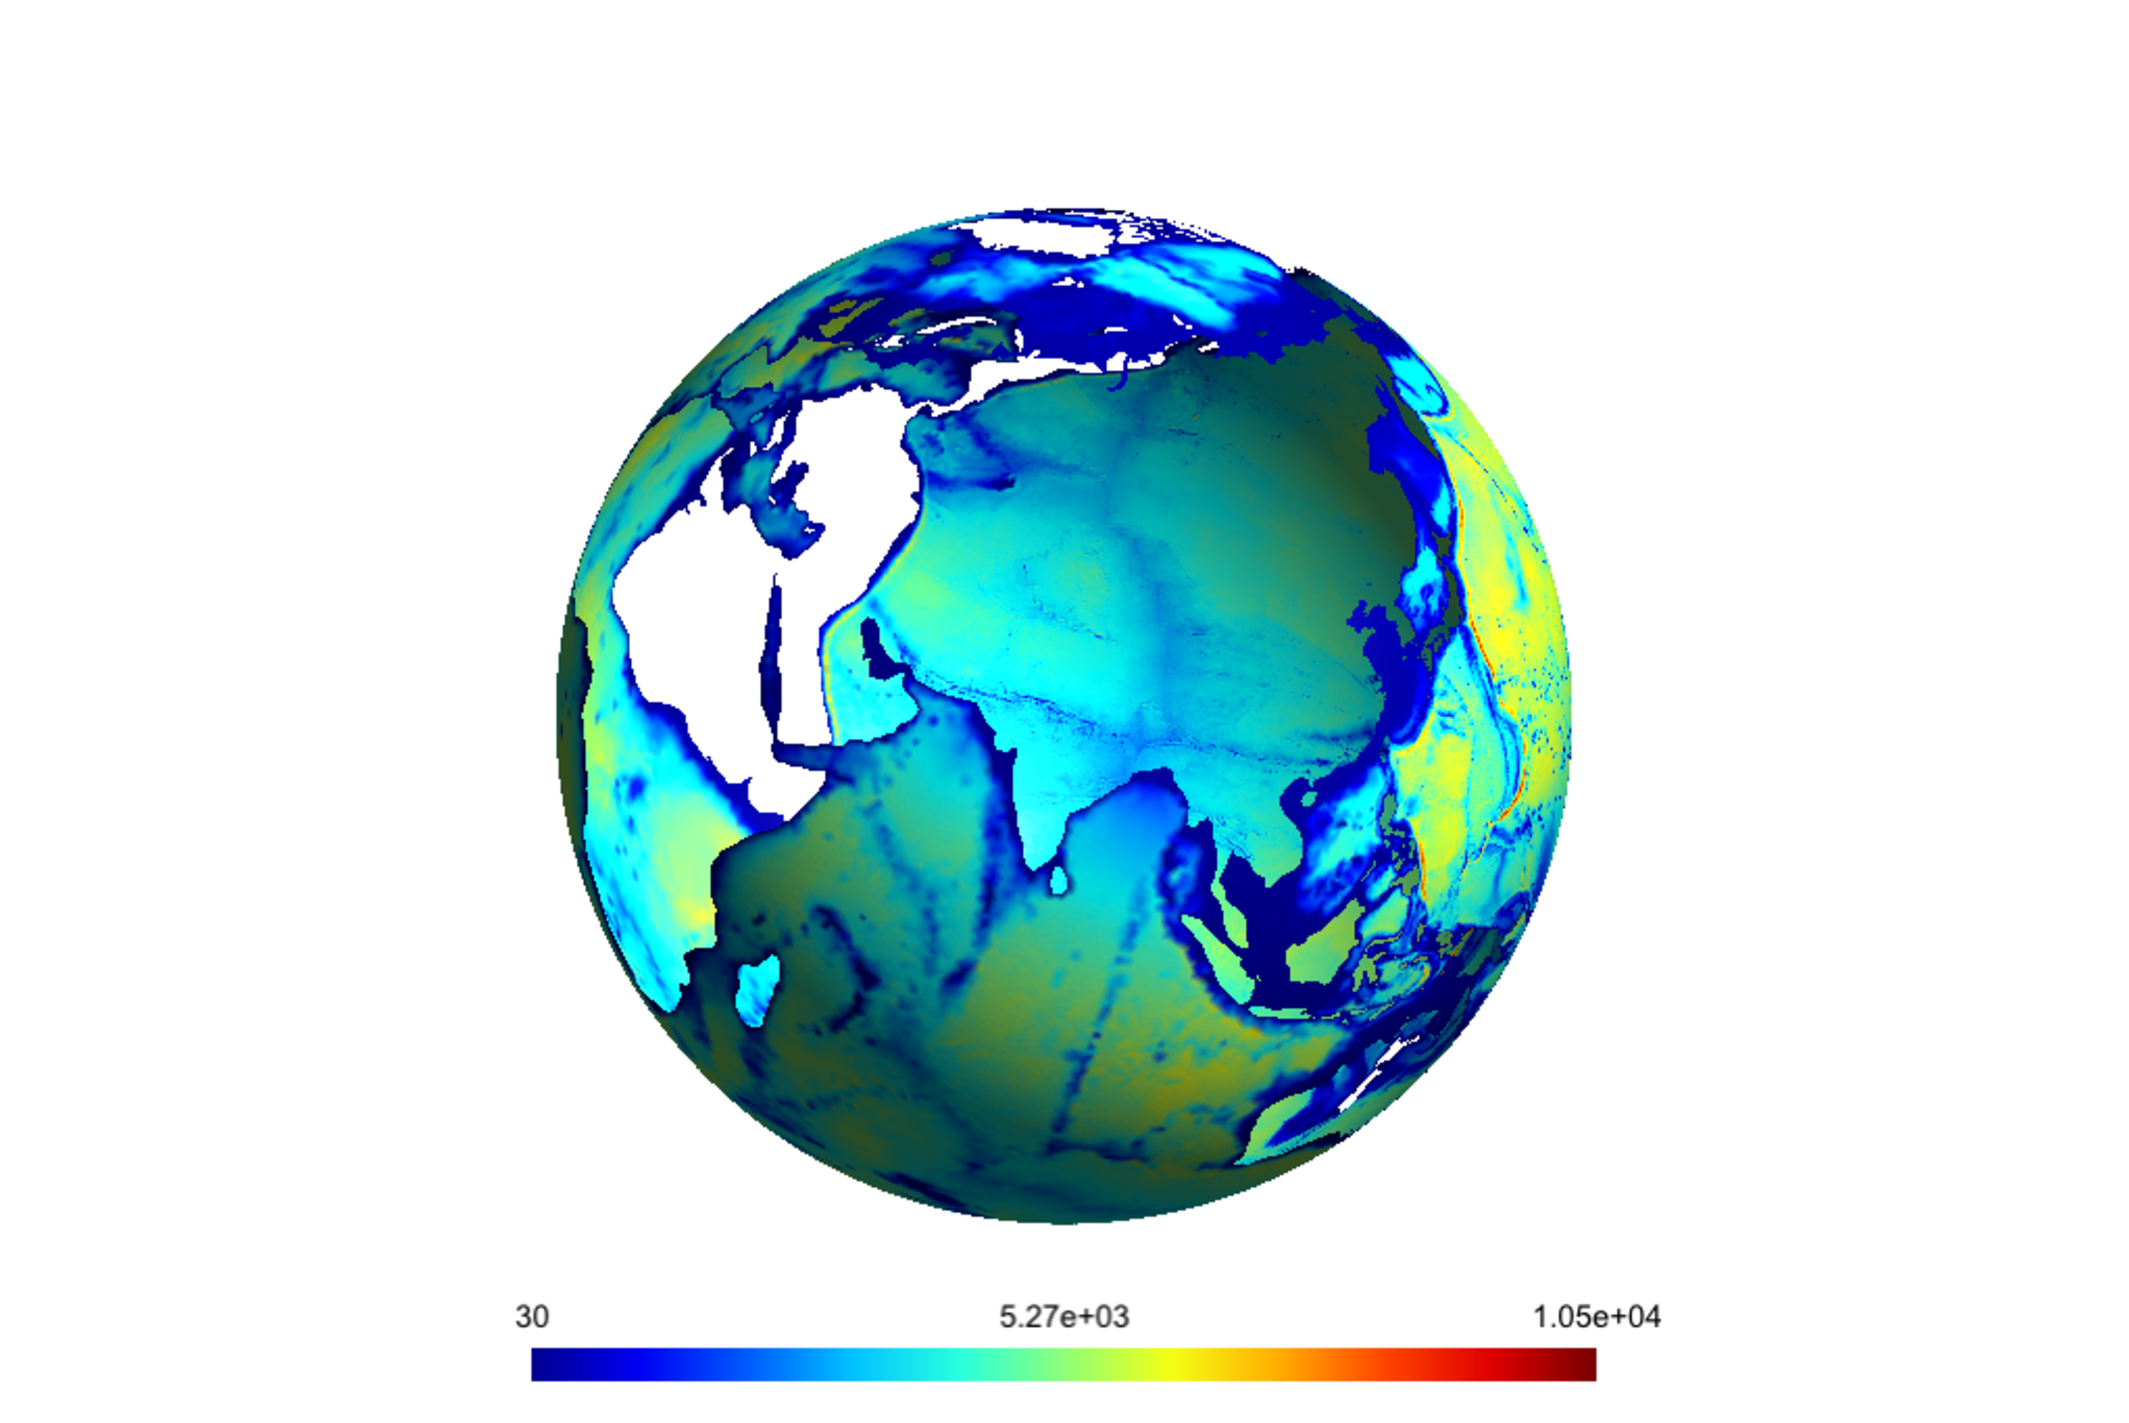
\includegraphics[trim=8cm 0cm 7cm 3cm,clip=true,width=0.5\linewidth]{./figures/globalOceanBathy.pdf}
\caption{\emph{Bathymetry distribution (in meters) in global ocean.}}
\label{fig:world_ocean_bathy}
\end{center}
\end{figure}

\subsection{Initial conditions}
Accurate representation of the initial wave generated after the earthquake event is required to simulate the wave propagation of the tsunami. In reality, the earthquake locations are not known and are estimated using several gauge recordings observed during the propagation of the wave (for an example,  see \cite{percival2011extraction}). For the validations, the initial surface displacement is estimated using the Okada model \cite{okada1992internal} and the earthquake data sets from United States Geological Services (USGS \cite{usgs}). The Okada model constructs the displacement of the seabed in the vertical direction, $Z$ at grid points ($X$, $Y$) using the fault plane parameters.

%The USGS earthquake data consists of five fault planes, given in Fig. (\ref{fig:indian_ocean_earth_quake}) \cite{ioualalen2007modeling}, that triggered Indian Ocean tsunami.  The vertical displacements due to each of these planes are obtained using Okada model and are aggregated to construct suitable initial conditions for forward wave propagation model. The constructed initial conditions are shown in Fig. (\ref{fig:indian_ocean_inc}). 

%\begin{figure}[h!]
%\begin{center}
%\centering
%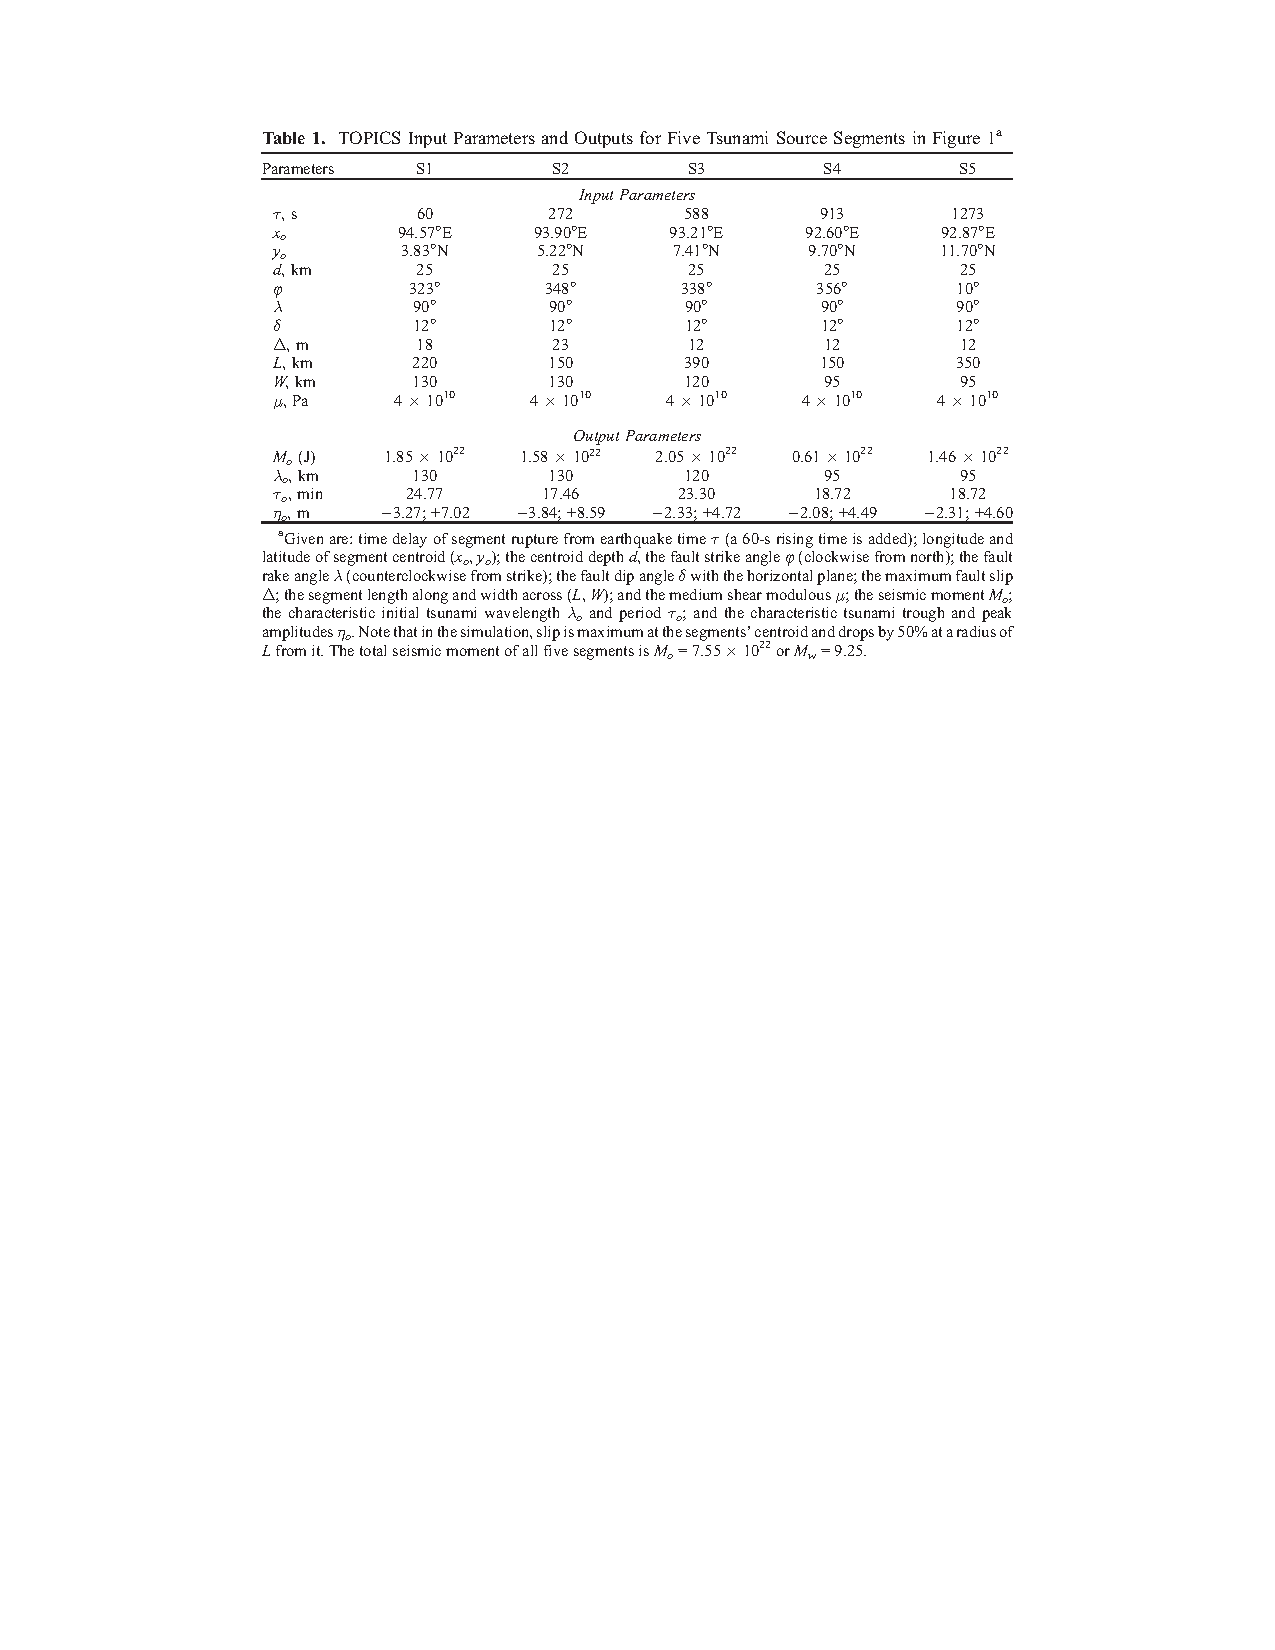
\includegraphics[trim=0cm 0cm 0cm 0cm,clip=true,width=\linewidth]{./figures/IndianOceanEarthQuake.pdf}
%\caption{\emph{Fault data of Sumatra earthquake. This  data is used as input for the Okada model to construct the initial displacement field of tsunami.}\cite{ioualalen2007modeling}}
%\label{fig:indian_ocean_earth_quake}
%\end{center}
%\end{figure}


\begin{figure}[h!]
\begin{center}
\centering
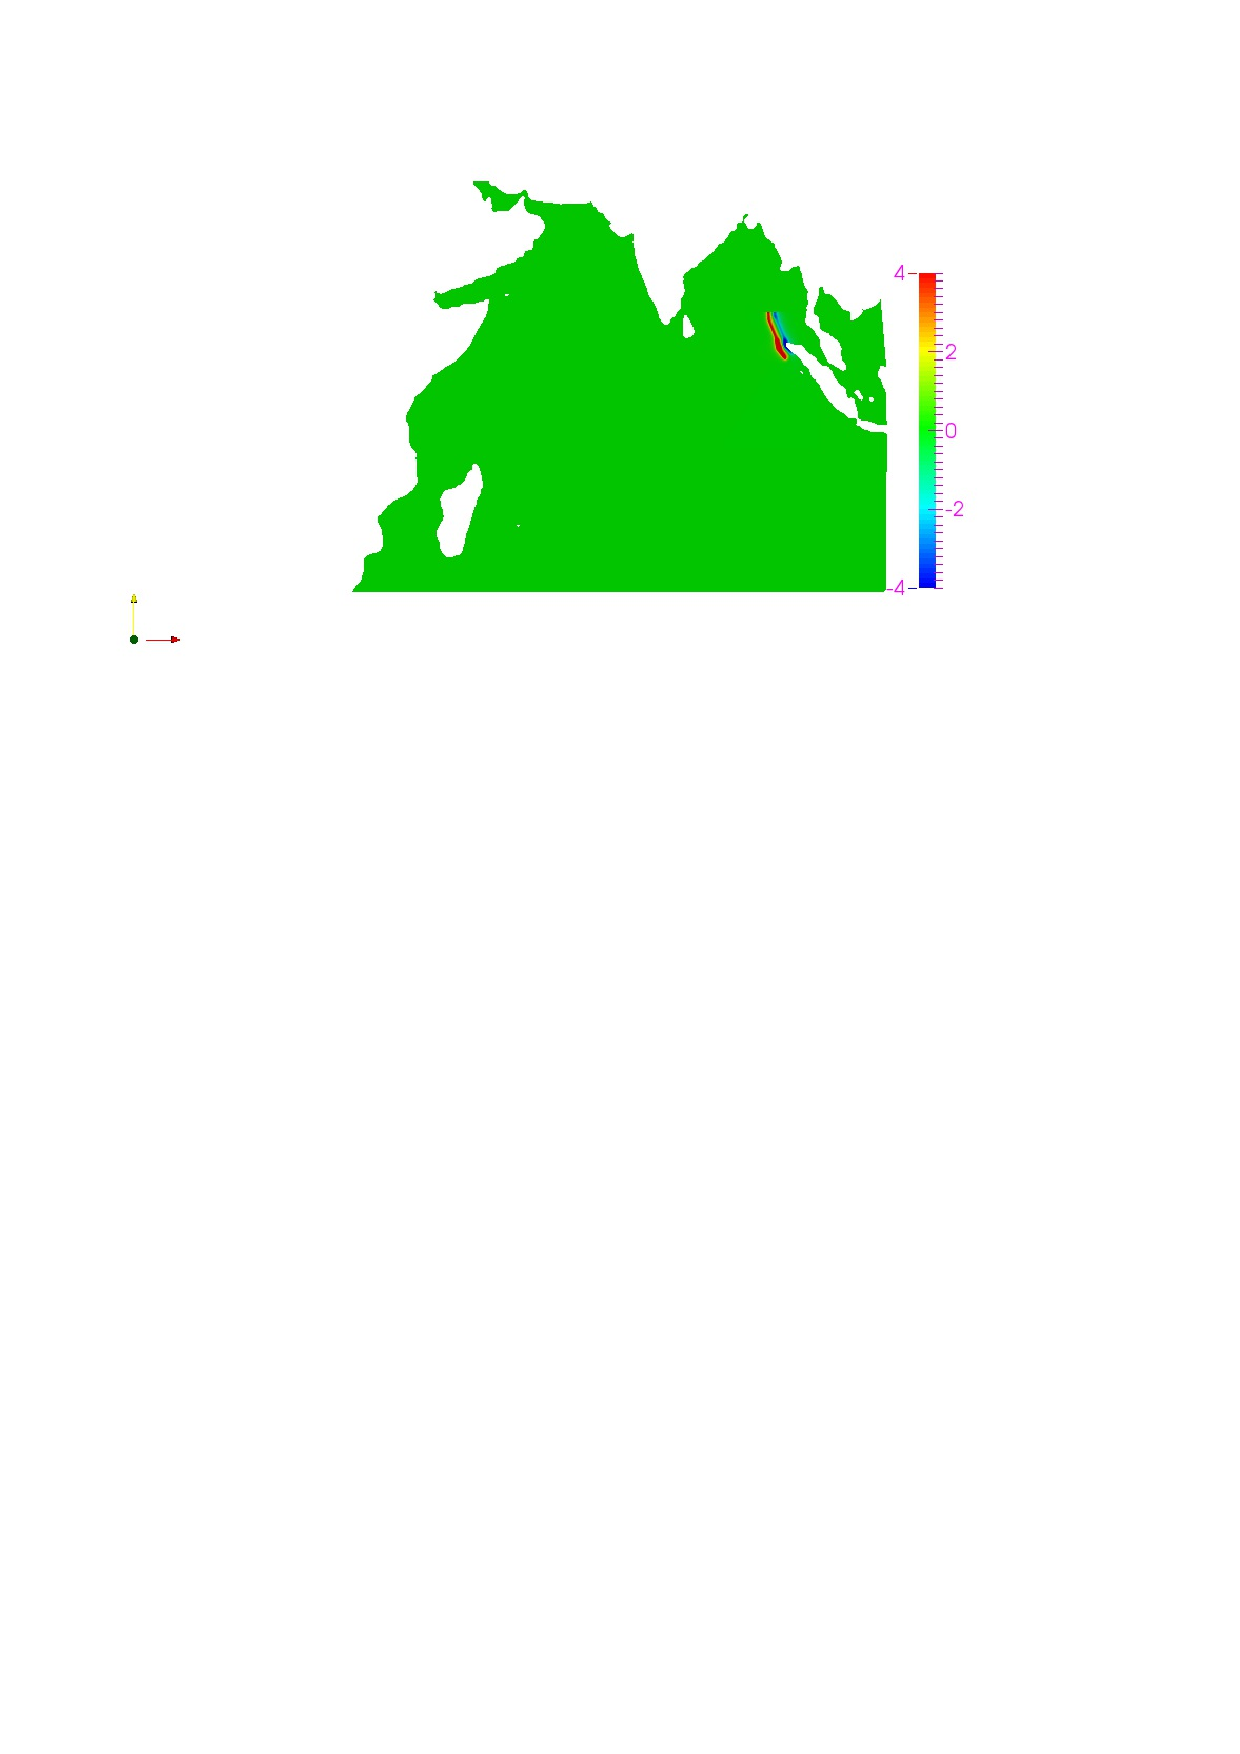
\includegraphics[trim=6cm 19.55cm 4.5cm 3cm,clip=true,width=0.5\linewidth]{./figures/IndianOceanINC.pdf}
\caption{\emph{Initial fluid displacement (in meters) from Okada model.}}
\label{fig:indian_ocean_inc}
\end{center}
\end{figure}

\subsection{Bottom friction}
Bottom friction force is parameterized by Ch\'ezy-Manning-Strickler formulation  \cite{gourgue2009flux} and is given by,
\begin{eqnarray}
\tau_{bx} &=& \frac{n^2 g}{h^{10/3}}\sqrt{(hu)^2+(hv)^2(}hu), \nonumber \\
\tau_{by} &=& \frac{n^2 g}{h^{10/3}}\sqrt{(hu)^2+(hv)^2}(hv)
\end{eqnarray}
here, $n$  is the Manning coefficient, an estimated roughness parameter of the ocean bed, is chosen to be $0.025~ s/m^{1/3}$, which is a typical value for sand. With the addition of the nonlinear forcing terms, the linear multi-rate time stepping is no longer stable. For the stability of the scheme the friction terms are integrated with implicit first order Euler method. The resulting scheme is an implicit-explicit time integration scheme. \begin{eqnarray}
\frac{dQ_H}{dt} &=& \mathcal{R}(Q_H) + S_b(Q_H),  \nonumber \\
Q_H^{n+1} -  \Delta t S_b\left(Q_{H} ^{n+1}\right) &=& Q_{H}^n + \sum_{i=0}^{2} \alpha_i\Delta t\mathcal{R}\left(Q_H ^{n-i}\right),
\end{eqnarray}
$S_b$ is the vector of bottom friction force, $Q_H ^n$ is the discrete solution at time step $n$, and  $\alpha_i$'s are coefficients of explicit multi-rate scheme. The above nonlinear system of equations is decoupled and point-wise. The exact solution of these equations can be obtained by solving a quadratic equation. However, the formula consists of a possibility of division with very small numbers, during the simulations. This leads to unstable rounding errors. Consequently, the nonlinear equations are linearized. %Consequently, these nonlinear equations are solved with Newton's method. The point-wise Jacobian matrix can be evaluated since the bottom friction is described by an analytical formula.

Adding the bottom friction is crucial near the shore where the fluid height is small. Fluid momentum builds up near shore and leads to large and unphysical velocities resulting in instabilities in the numerical solution. This instability is predominant for high order discretizations. Friction terms stabilize the flow in these regions and ensure the velocities to be bounded \cite{leveque2011tsunami}. 

\subsection{Boundary conditions}
Reflecting boundary conditions are imposed on the coastal boundary. However, the boundary conditions near the artificial boundary where the physical domain is truncated to a particular region of interest, is not straight forward. The artificial boundary reflects the outgoing waves into the physical domain. Thin sponge/absorbing layers are added near these boundaries \cite{modave2010parameters} to minimize these reflections. In these layers the numerical solution is nudged towards the exterior solution (zero in this context) by introducing a damping term in the PDE in these layers. We do not use the reflecting boundary conditions for the simulation in the world ocean since there are no unphysical boundaries. 

%The modified PDE in absorbing layers is given by,
%\begin{eqnarray}
%\frac{\partial \eta}{\partial t} + \frac{\partial F_1}{\partial x} + \frac{\partial G_1}{\partial y} &=& -(\sigma_x +\ \sigma_y) \eta, \nonumber \\
%\frac{\partial (hu)}{\partial t} +\ \frac{\partial F_2}{\partial x} + \frac{\partial G_2}{\partial y} &=& S_2 + \tau_{bx} - \sigma_x hu, \nonumber \\
%\frac{\partial (hv)}{\partial t} +\ \frac{\partial F_3}{\partial x} + \frac{\partial
%G_3}{\partial y} &=& S_3 + \tau_{by} - \sigma_y hv,
%\end{eqnarray}
%here, $\sigma_x$ and $\sigma_y$ are optimal damping coefficients derived for linear gravity waves. For one dimensional problem the coefficient $\sigma$ in the absorbing layer is given as,
%\begin{equation}
%\sigma(x) = \frac{\sqrt{gh}}{\delta} \frac{x}{\delta - x}, 
%\end{equation}
%here, $x$ is the distance from the outflow boundary and $\delta$ is the thickness of the absorbing layer. $\delta$ has to be sufficiently large in order to get significant damping of the outgoing waves in the absorbing layer. 

\subsection{Multi-rate time stepping}
At the beginning of the simulation, the elements are grouped into levels for the multi-rate time scheme, based on the elemental CFL condition. Fig (\ref{fig:indian_ocean_levels}), shows the distribution of the multi-rate levels for this simulation. Table (\ref{tab:pasidgLevels}), shows the percentage of elements grouped into each level.  From the figure it is clear that the elements near the shore are grouped into levels $3$ and $4$, that are the finest levels in the multi-rate scheme, whereas the elements in deep ocean are grouped in to levels $1$ and $2$, that are the coarsest levels. Only $2\%$ of the overall elements fall in to the finest level, resulting in $98\%$ of the elements requiring at most half of the computations when compared to a single rate scheme.

\begin{table}[h!]
\begin{center}
\begin{tabular}{crrrrr}
\hline
Level & \# elements & \% of elements & work per elem & \% of overall work\\ \hline
1 &  9960 &  7.63 & 1 & 2.60\\
2 & 60123 &  46.09 & 2 & 31.37\\
3 & 57441 & 44.04 & 4 & 59.94\\
4 &  2920 &  2.24 & 8 & 6.09\\\hline
\end{tabular}
\caption{\emph{Distribution of time stepping levels in multi-rate time integration
scheme.}}
\label{tab:pasidgLevels}
\end{center}
\end{table}
\begin{figure}[h!]
\begin{center}
%\centering
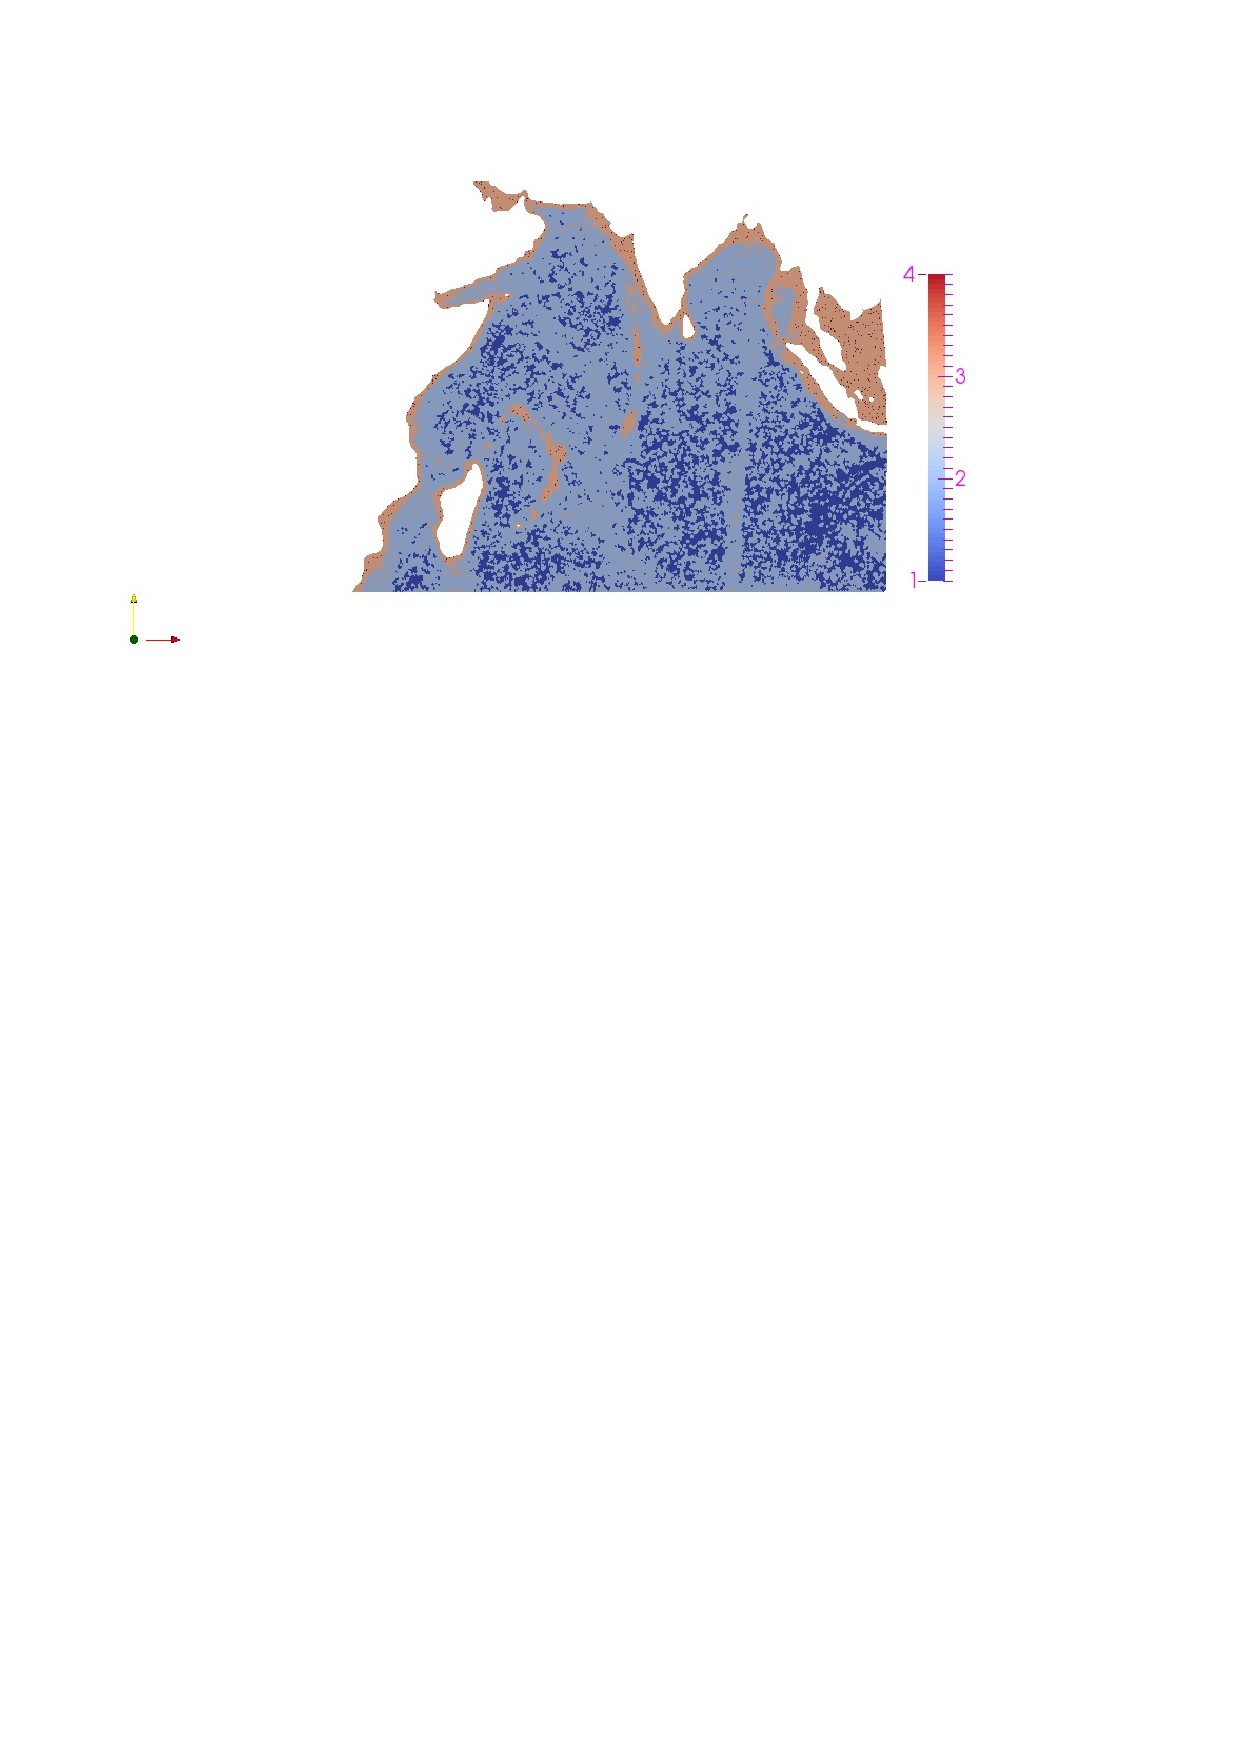
\includegraphics[trim=6cm 19.65cm 4.5cm 3.1cm,clip=true,width=0.5\linewidth]{./figures/IndianOceanLevels.pdf}
\caption{\emph{Distribution of  multi-rate levels for time stepping with
four levels.}}
\label{fig:indian_ocean_levels}
\end{center}
\end{figure}


\section{Results: Indian Ocean tsunami}
\label{sec:results}
In this section, we compare the simulation results with recorded data of Indian Ocean tsunami. However, we do not compare the simulation results of the Japan tsunami. We that case study to demonstrate the performance.  
\subsection{Tidal gauge comparisons}
The numerical solutions are verified with the tide gauge records found in  \cite{gaugerecords}. Some of the previous work on validation using DGCOM \cite{gopalakrishnan2011tsunami} for Indian Ocean tsunami without a positivity preserving limiter is found in Alveras thesis \cite{alevras2009simulating}.

The important feature is the arrival time of the tsunami wave. The time at which the first peak in the elevation is observed, is considered to be the arrival time of a tsunami wave. Fig (\ref{fig:gauge_compare}), compares the simulation results with tidal gauge measurements at Chennai, Tuticorin, Mormugao, and Okha stations in India. The numerical model predicts the arrival times very accurately while the time history of the fluid heights estimated does not match the records exactly. 
\begin{figure}%[h!]
\begin{center}
  \subfloat[Chennai ($80.30^0 E$, $13.10^0 N$)]{%
    \begin{minipage}[c]{0.45\linewidth}
      \centering%
      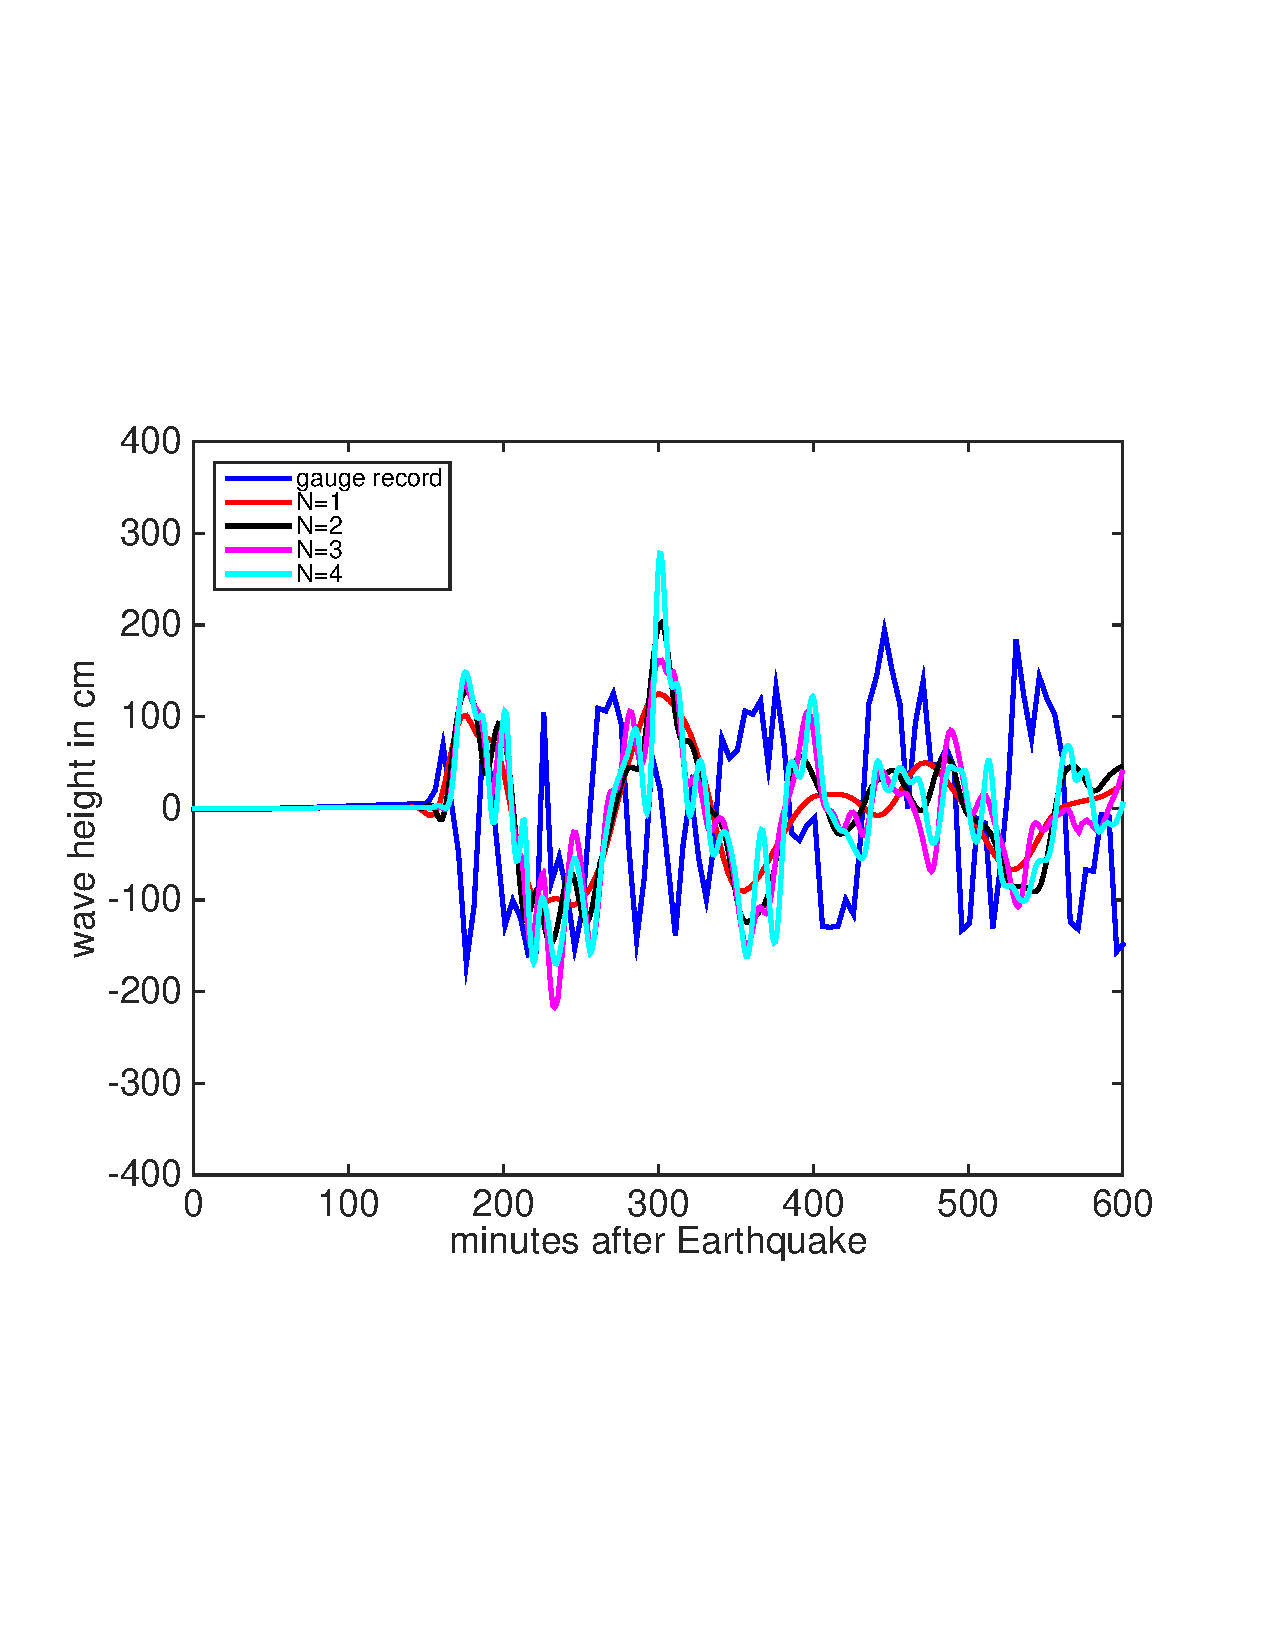
\includegraphics[trim=0cm 6cm 2cm 7cm,clip=true,width=\textwidth]{./figures/chennaiGaugeCon.pdf}
  \end{minipage}} \hspace{0.5cm}
  \subfloat[Tuticorin ($78.15^0 E$, $08.80^0 N$)]{%
    \begin{minipage}[c]{0.45\linewidth}
      \centering%
      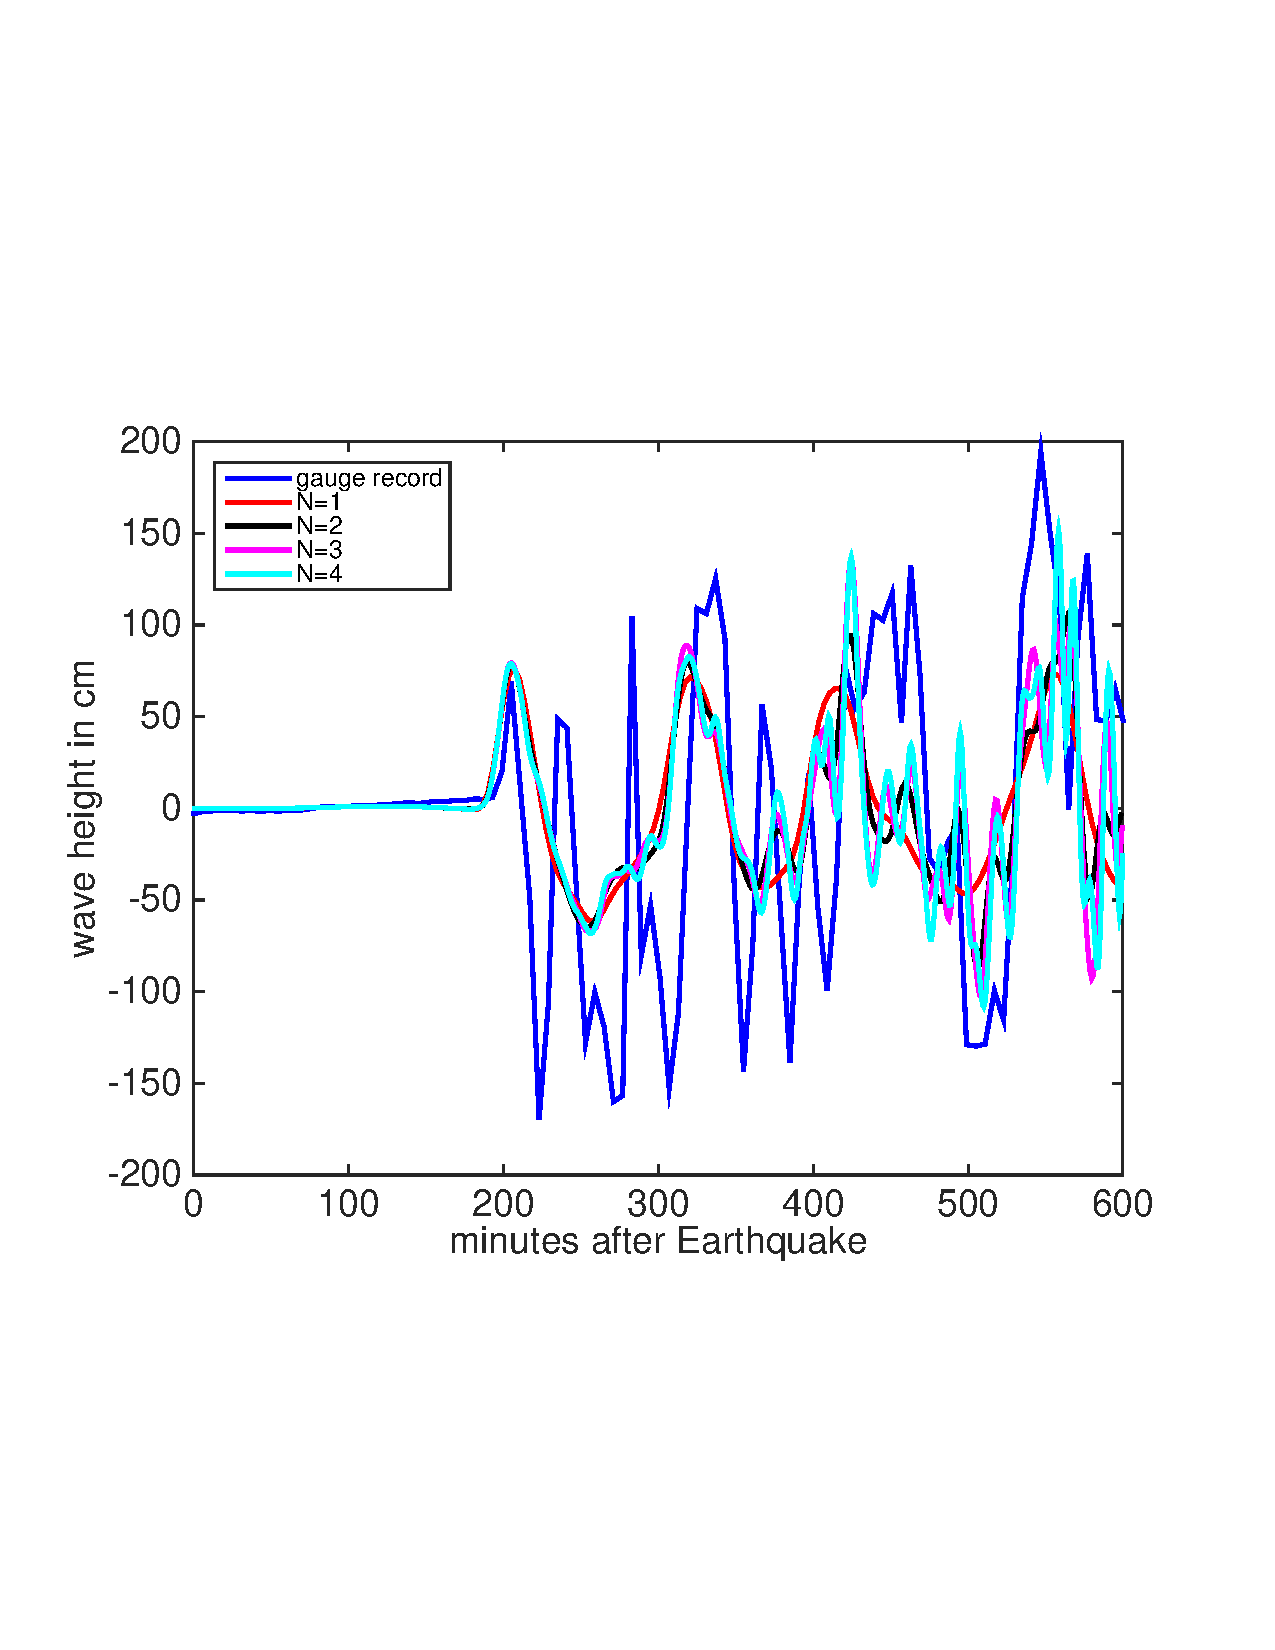
\includegraphics[trim=0cm 6cm 2cm 7cm,clip=true,width=\textwidth]{./figures/tuticorinGaugeCon.pdf}
  \end{minipage}}\\
    \subfloat[Mormugao ($73.80^0 E$, $15.42^0 N$)]{%
    \begin{minipage}[c]{0.45\linewidth}
      \centering%
      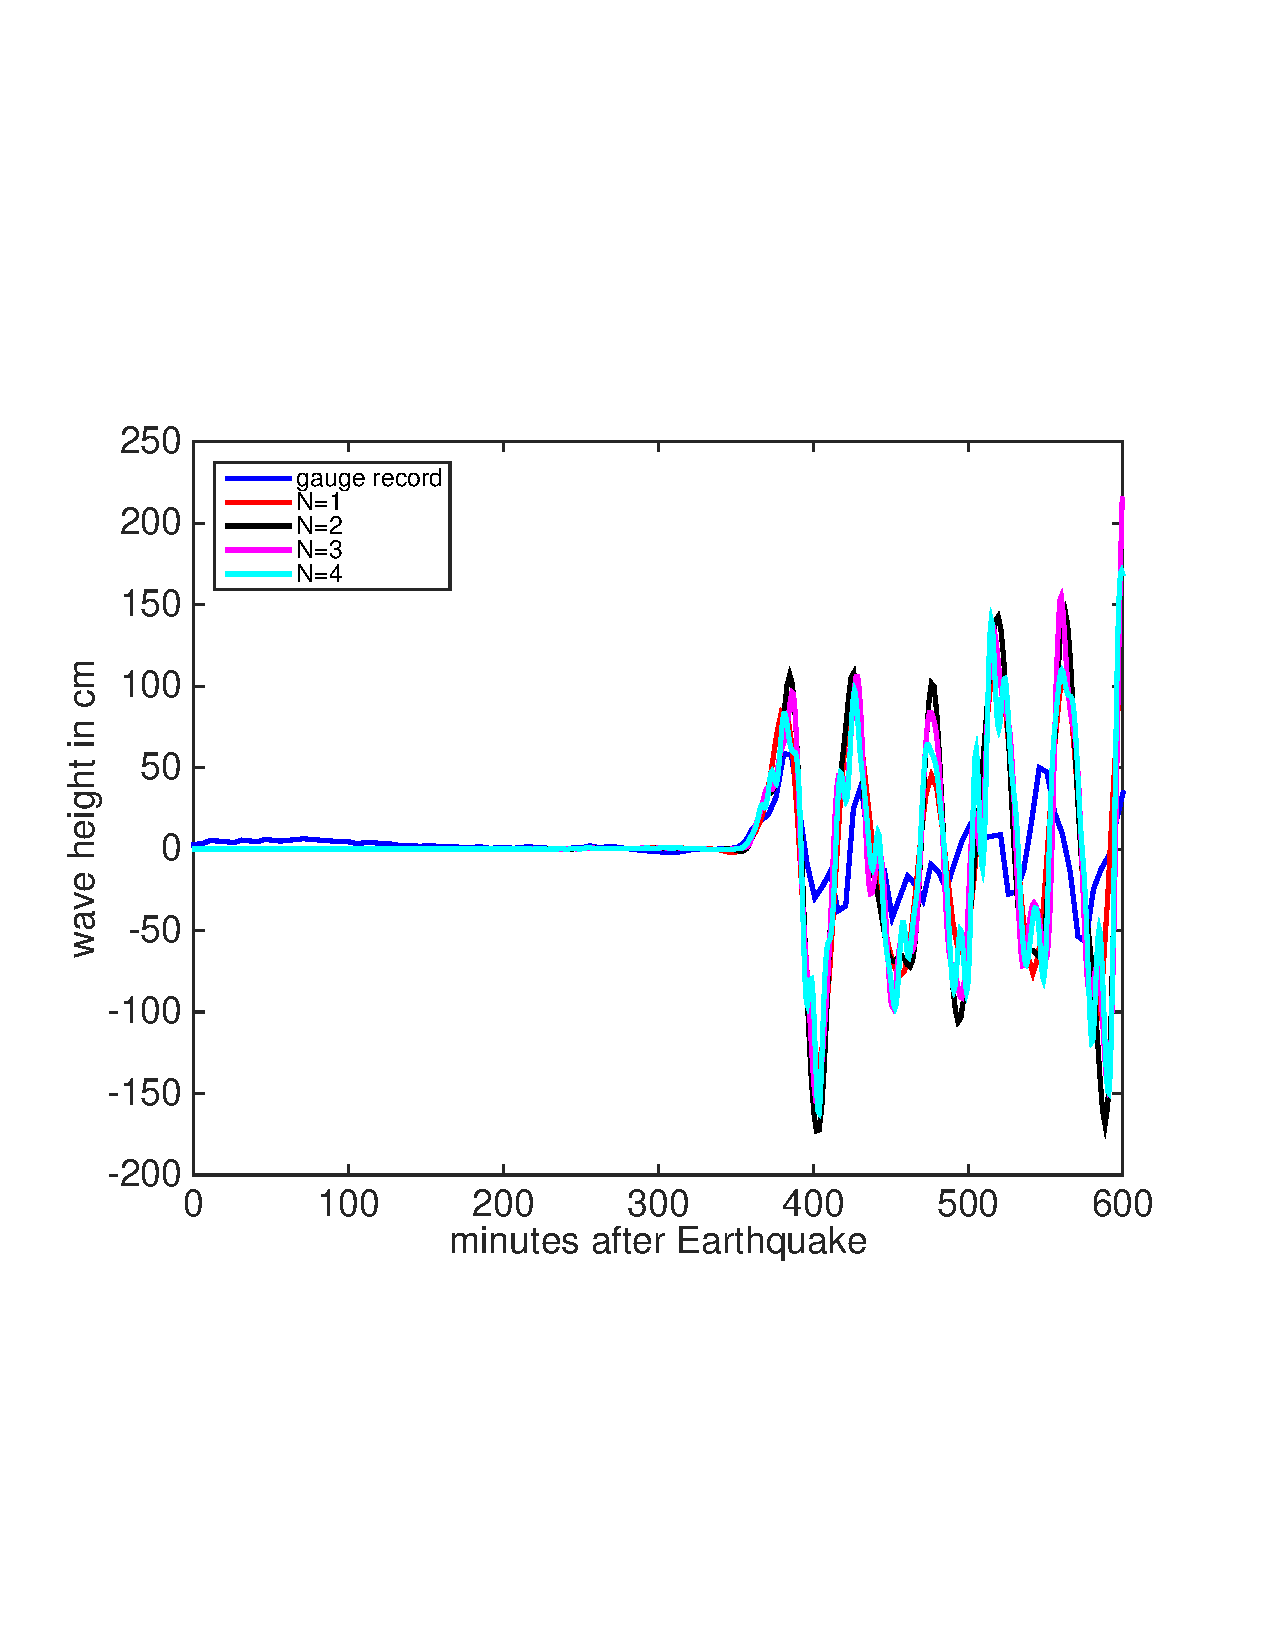
\includegraphics[trim=0cm 6cm 2cm 7cm,clip=true,width=\textwidth]{./figures/mormugaoGaugeCon.pdf}
  \end{minipage}} \hspace{0.5cm}
  \subfloat[Okha ($69.08^0 E$, $22.47^0 N$)]{%
    \begin{minipage}[c]{0.45\linewidth}
      \centering%
      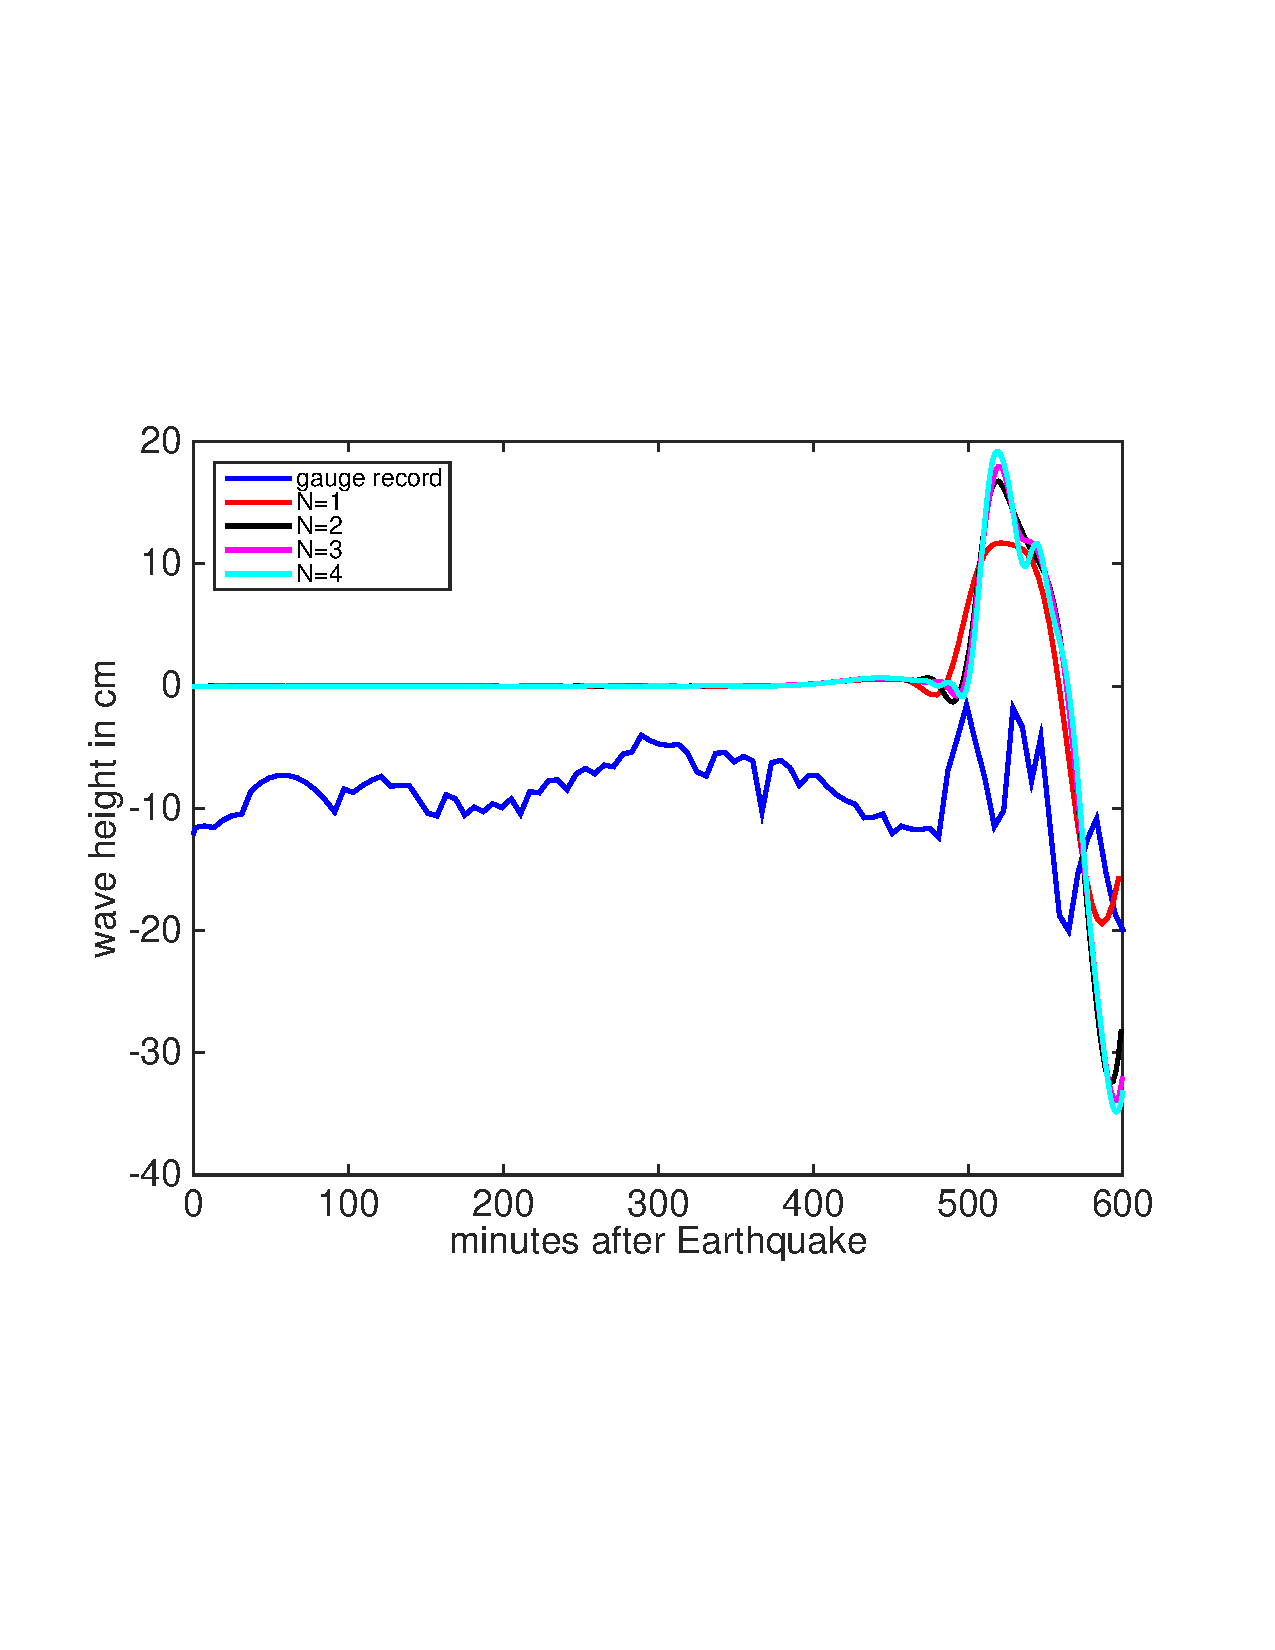
\includegraphics[trim=0cm 6cm 2cm 7cm,clip=true,width=\textwidth]{./figures/okhaGaugeCon.pdf}
  \end{minipage}}
\end{center}
 \caption{\emph{Comparison of simulation results with tidal gauge measurements at Chennai, Tuticorin, Mormugao, and Okha stations  in India.}}
  \label{fig:gauge_compare}
\end{figure}

\subsection{Fluid profile}
Fig (\ref{fig:tsunami_propagation}) shows the distribution of free surface elevation at $20$, $40$, $80$, and $160$ minutes after the Sumatra earthquake. These results are comparable with the results obtained  using ICOM \cite{pietrzak2007defining}.
In Fig (\ref{fig:tsunami_propagation_compare_N}), we show the free surface obtained at $80$ minutes using the simulation with approximation orders $1$ to $4$. These results are qualitatively similar. It might be due to the low resolution (linear in each triangle) of bathymetry distribution used.

\begin{figure}%[h!]
\begin{center}
  \subfloat[Free surface elevation at 20 min]{%
    \begin{minipage}[c]{0.45\linewidth}
      \centering%
      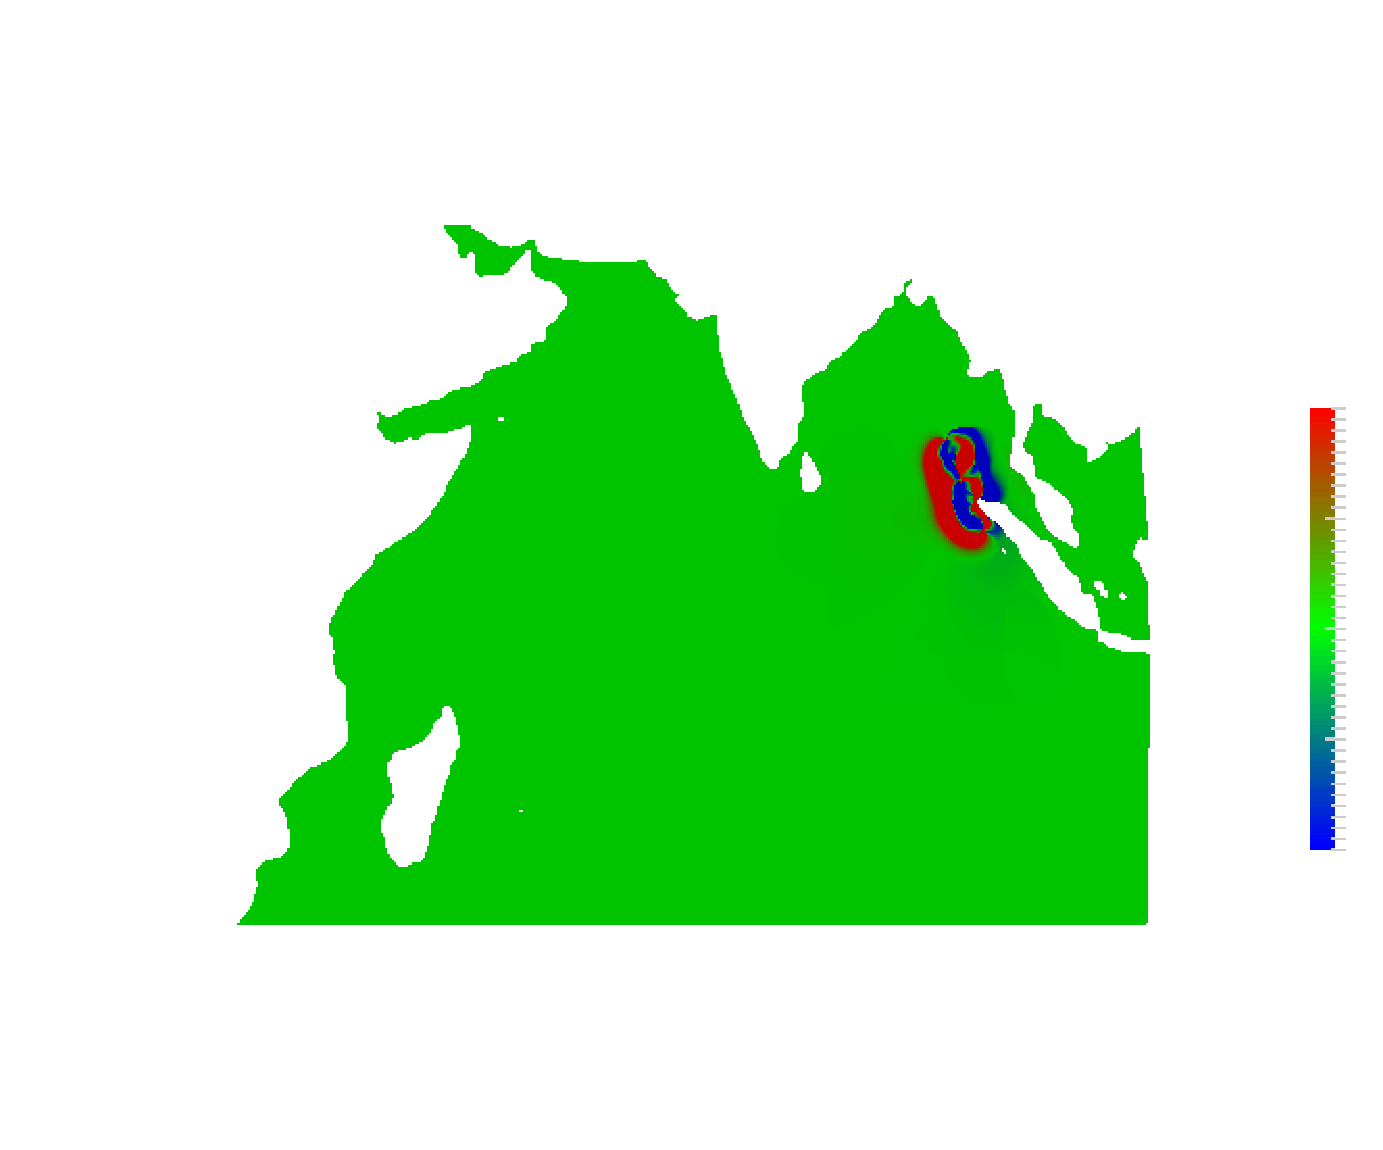
\includegraphics[trim=3.95cm 3.95cm 3.95cm 3.95cm,clip=true,width=\textwidth]{./figures/T20N4.pdf}
  \end{minipage}} \hspace{0.5cm}
  \subfloat[Free surface elevation at 40 min]{%
    \begin{minipage}[c]{0.45\linewidth}
      \centering%
      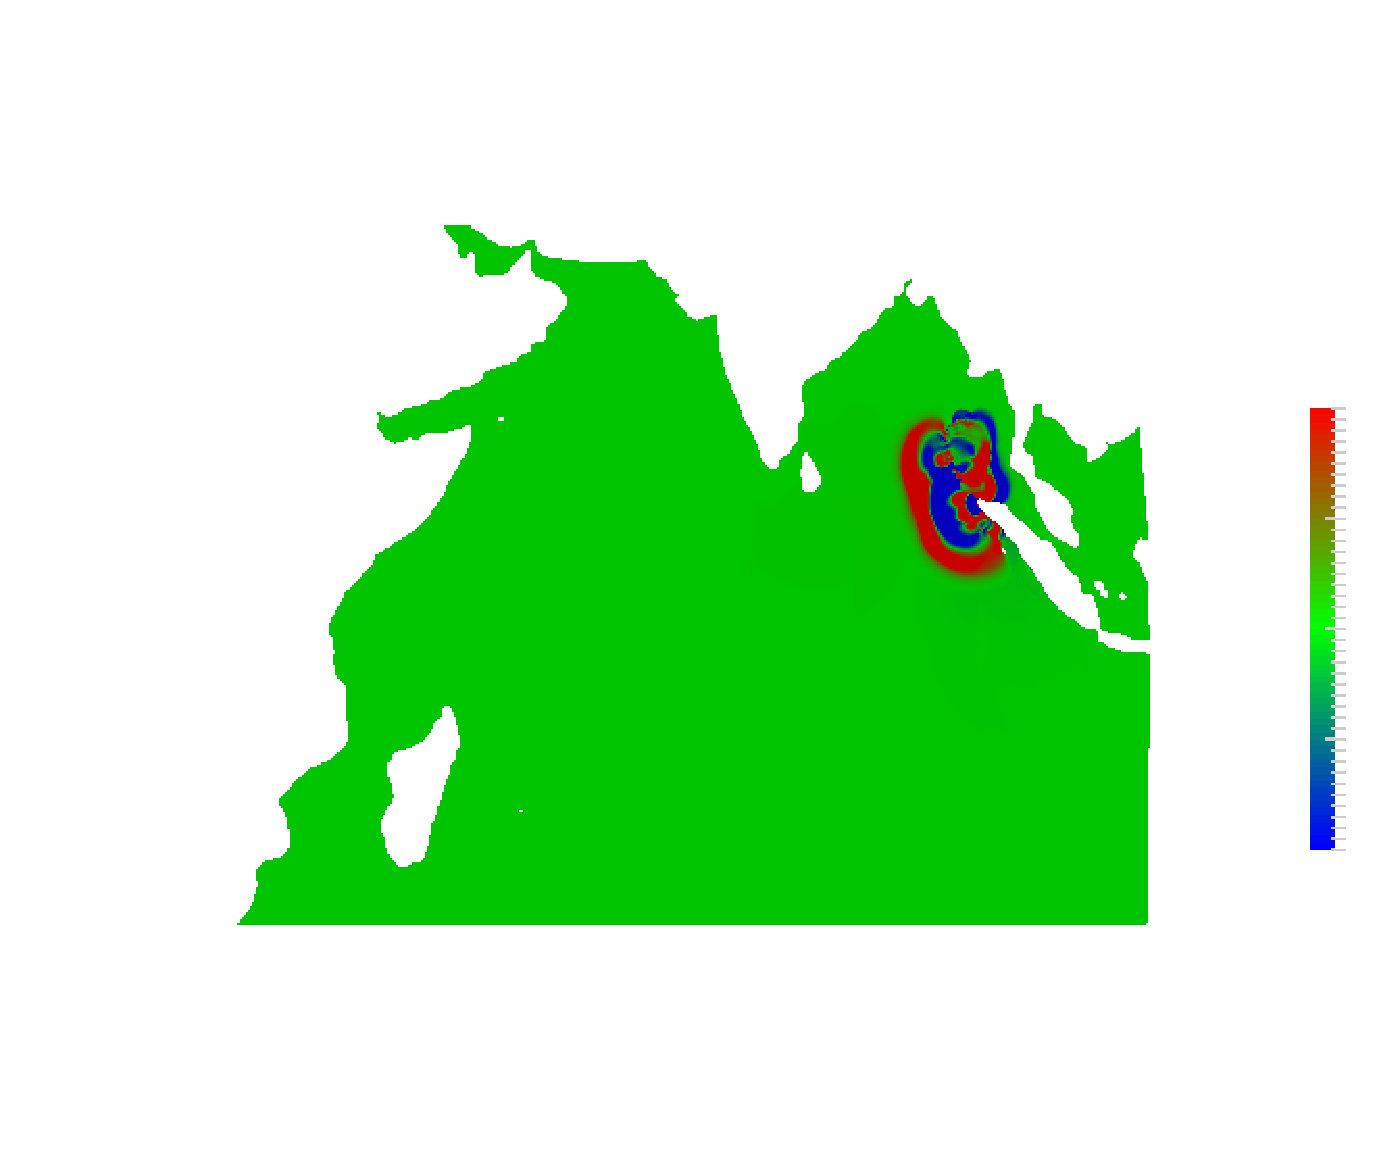
\includegraphics[trim=3.95cm 3.95cm 3.95cm 3.95cm,clip=true,width=\textwidth]{./figures/T40N4.pdf}
  \end{minipage}}\\
    \subfloat[Free surface elevation at 80 min]{%
    \begin{minipage}[c]{0.45\linewidth}
      \centering%
      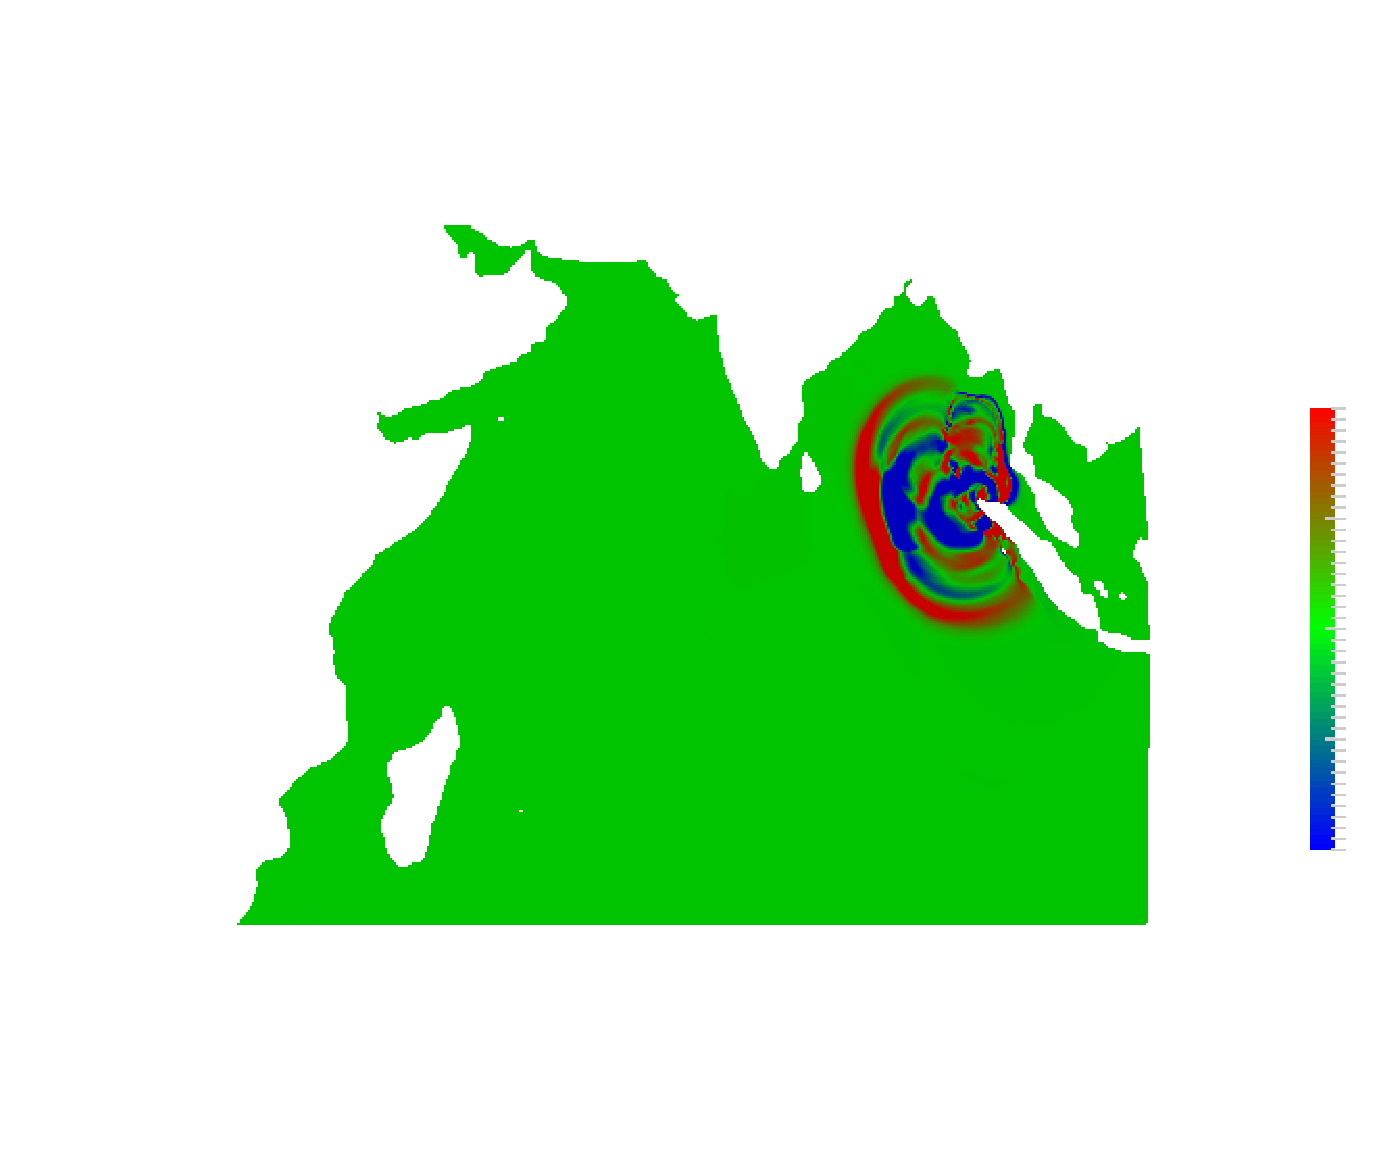
\includegraphics[trim=3.95cm 3.95cm 3.95cm 3.95cm,clip=true,width=\textwidth]{./figures/T80N4.pdf}
  \end{minipage}} \hspace{0.5cm}
  \subfloat[Free surface elevation at 160 min]{%
    \begin{minipage}[c]{0.45\linewidth}
      \centering%
      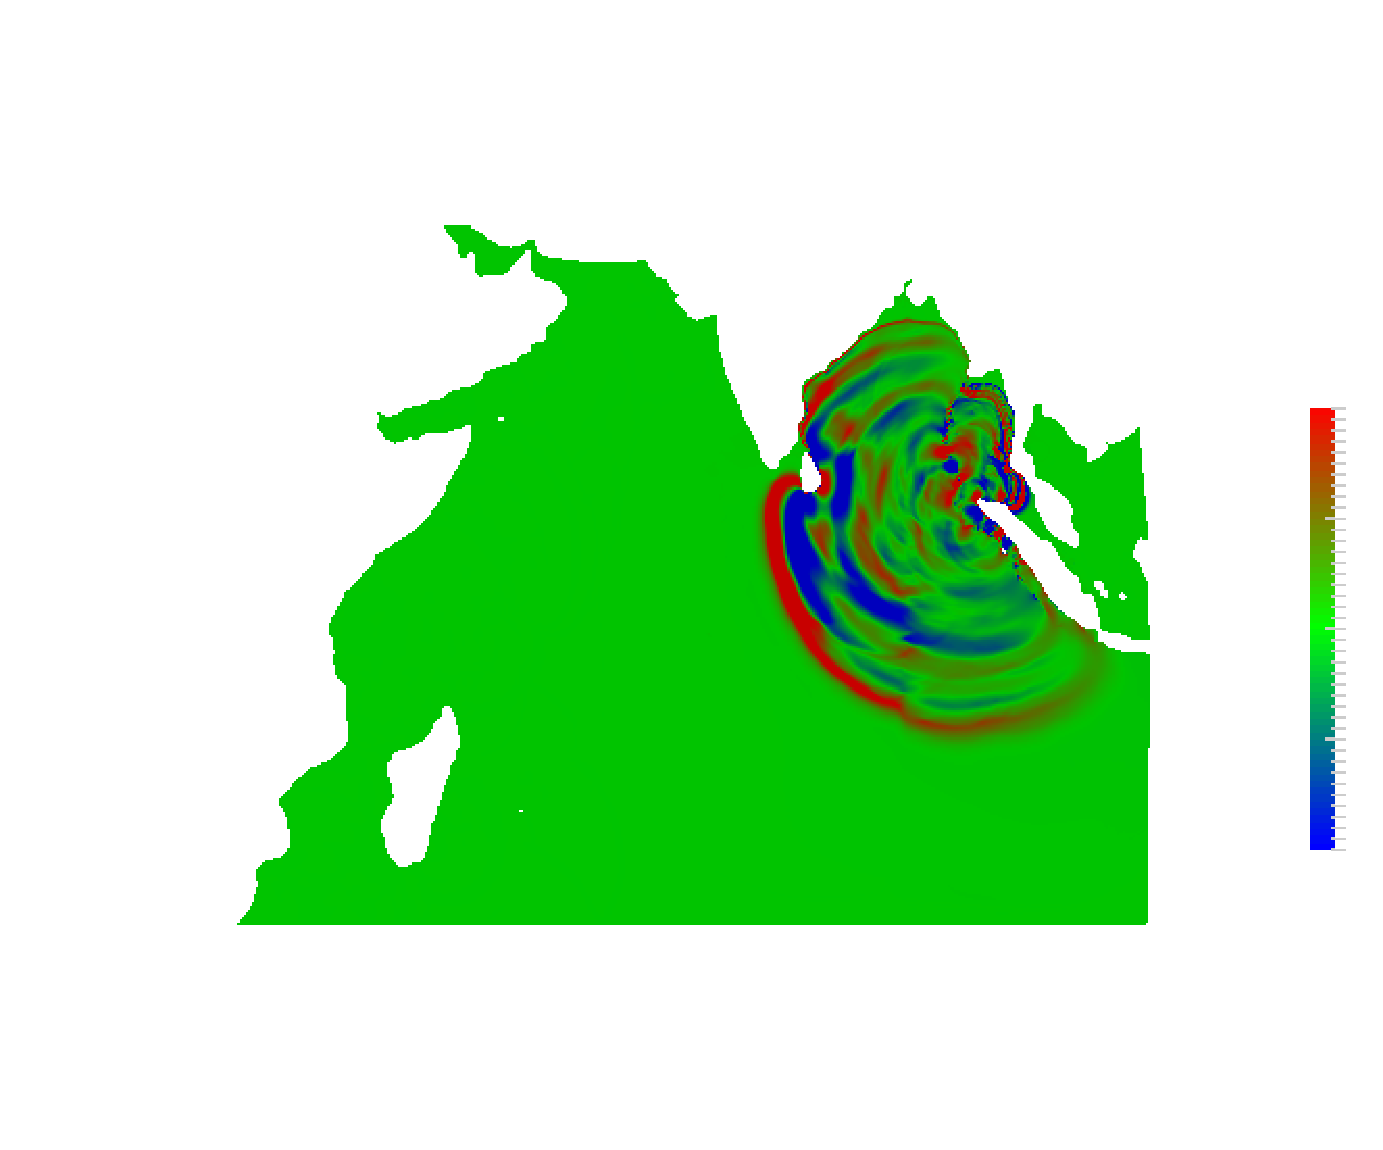
\includegraphics[trim=3.95cm 3.95cm 3.95cm 3.95cm,clip=true,width=\textwidth]{./figures/T160N4.pdf}
  \end{minipage}}\\
  \centering
   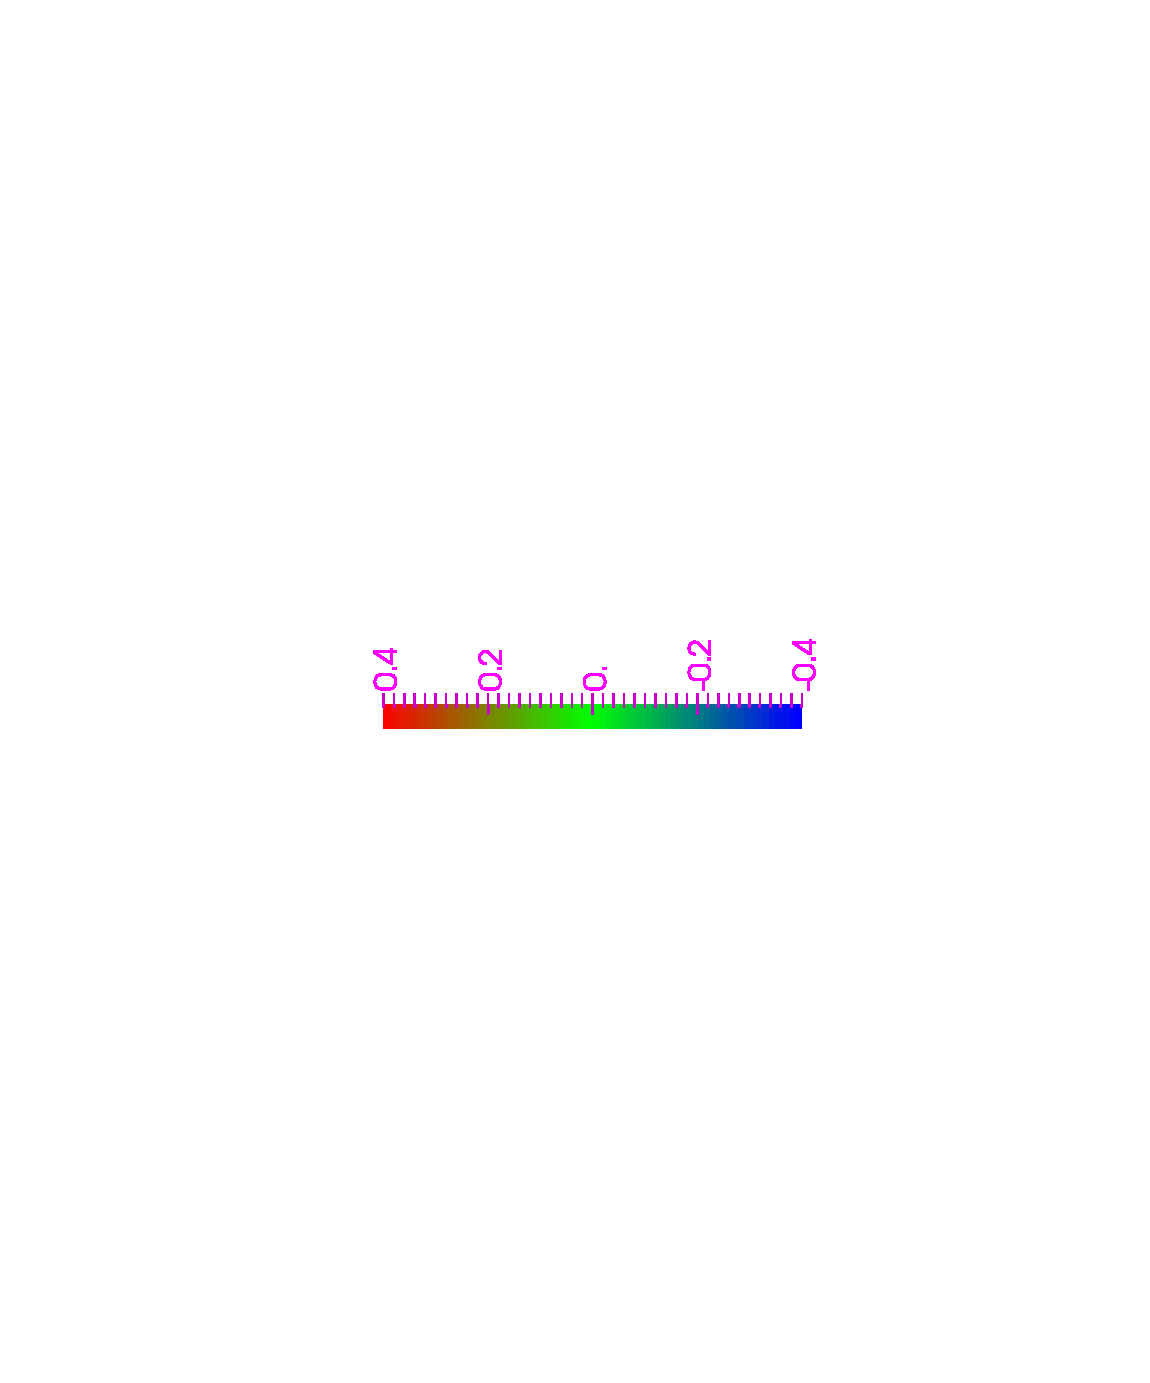
\includegraphics[trim=6cm 11cm 5cm 10.5cm,clip=true,width=0.5\textwidth]{./figures/TsunamiLegend.pdf}
\end{center}
 \caption{\emph{Free surface elevation of Indian Ocean tsunami at $20$, $40$,
$80$, and $160$ minutes after earthquake. Simulations are run with $4^{th}$
order polynomial approximation in each triangle with double precision arithmetic.}}
  \label{fig:tsunami_propagation}
\end{figure}

\begin{figure}%[h!]
\begin{center}
  \subfloat[N=1]{%
    \begin{minipage}[c]{0.45\linewidth}
      \centering%
      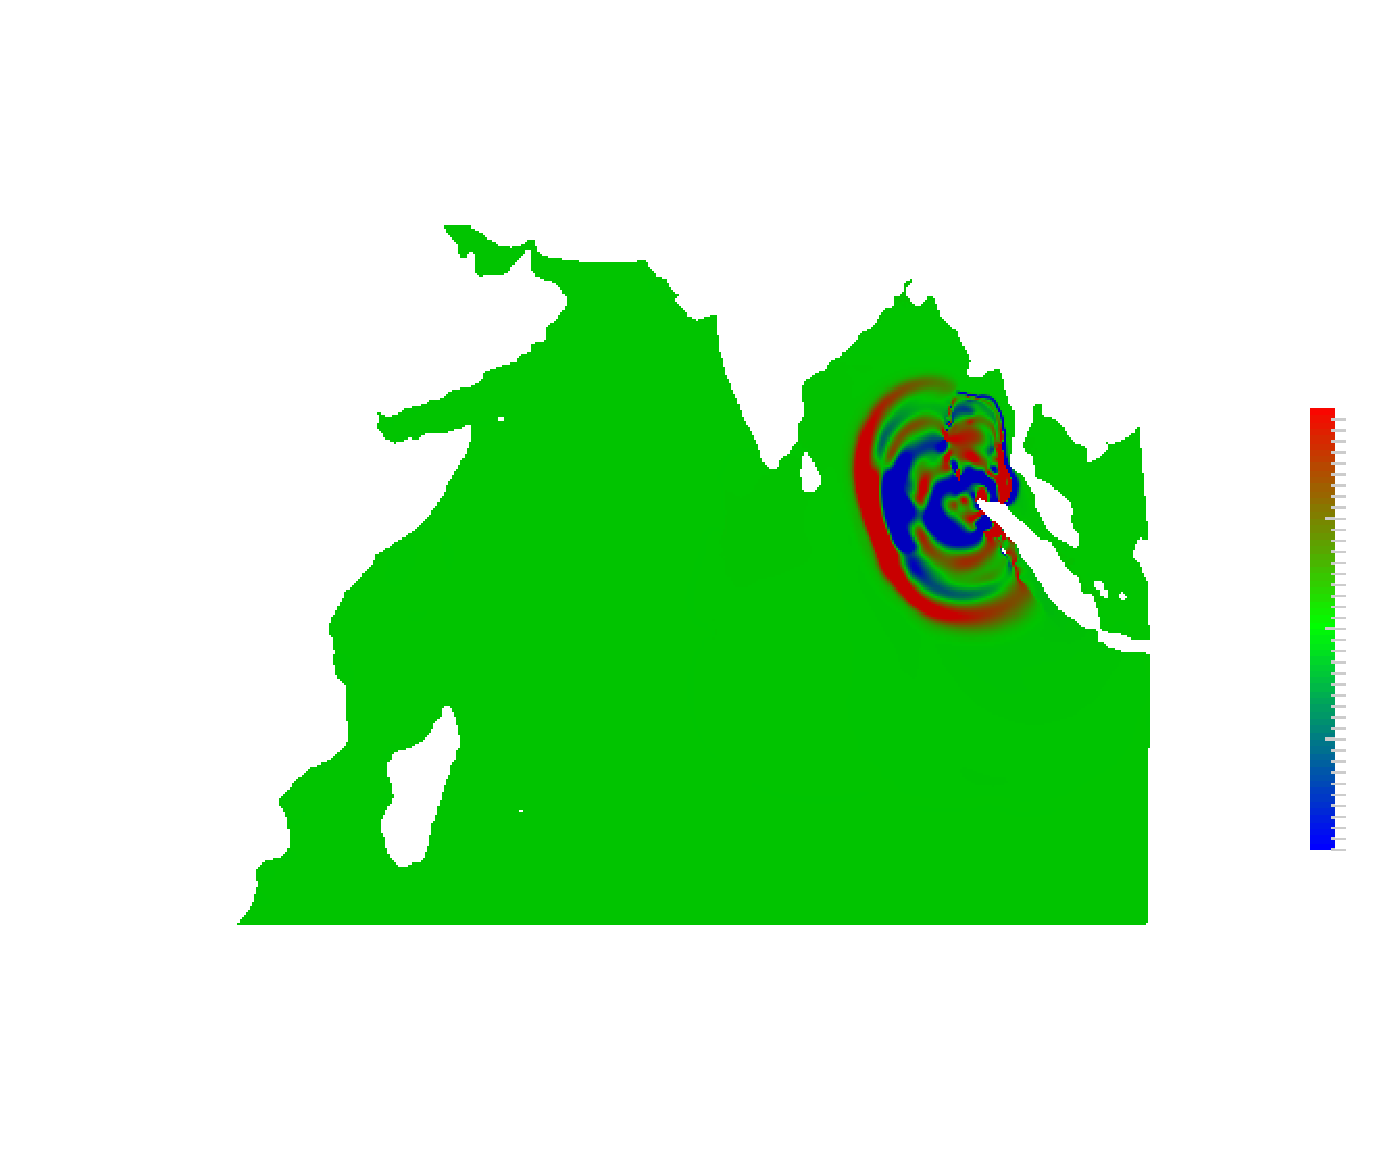
\includegraphics[trim=3.95cm 3.95cm 3.95cm 3.95cm,clip=true,width=\textwidth]{./figures/T80N1.pdf}
  \end{minipage}} \hspace{0.5cm}
  \subfloat[N=2]{%
    \begin{minipage}[c]{0.45\linewidth}
      \centering%
      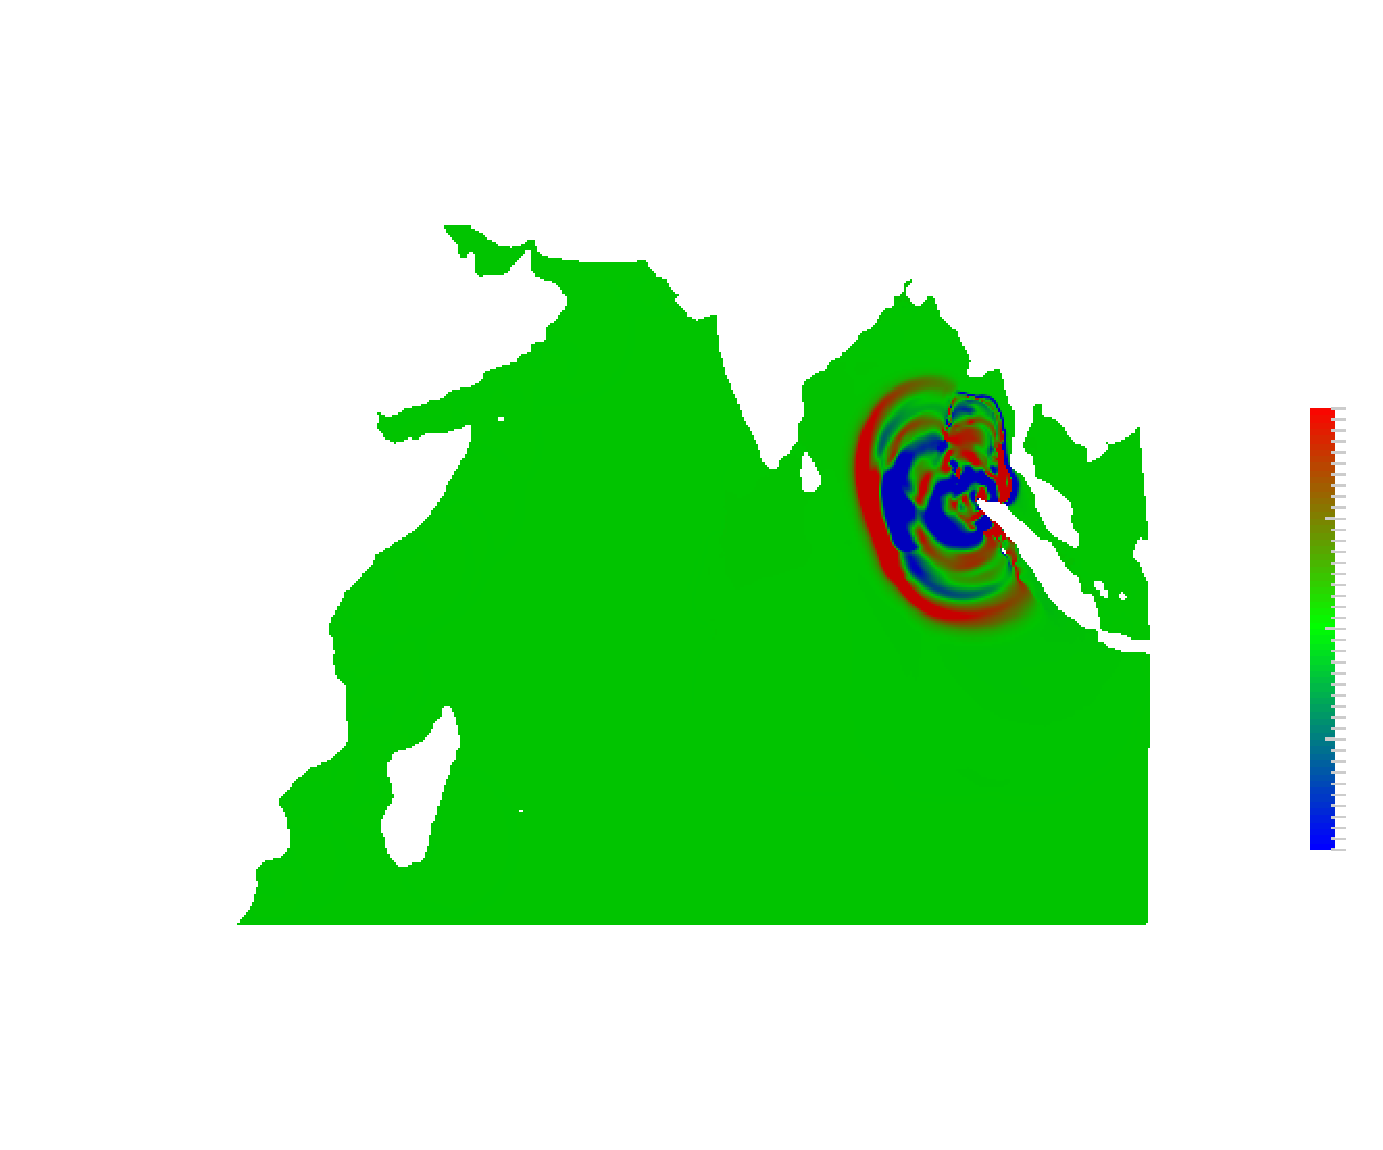
\includegraphics[trim=3.95cm 3.95cm 3.95cm 3.95cm,clip=true,width=\textwidth]{./figures/T80N2.pdf}
  \end{minipage}}\\
    \subfloat[N=3]{%
    \begin{minipage}[c]{0.45\linewidth}
      \centering%
      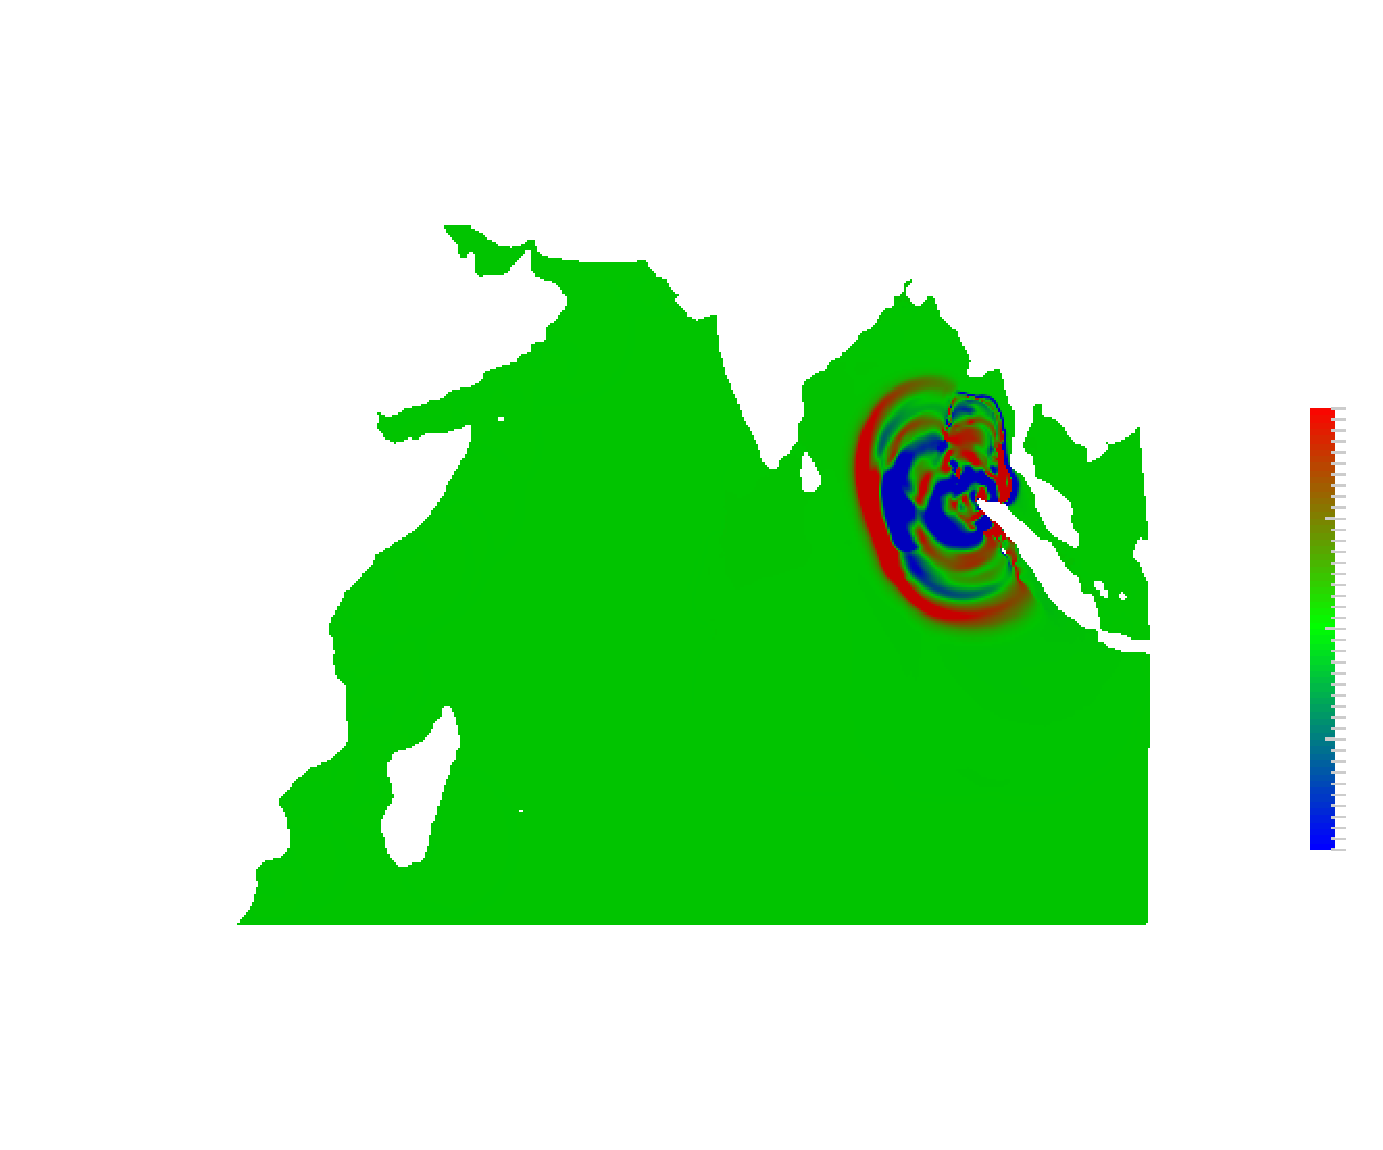
\includegraphics[trim=3.95cm 3.95cm 3.95cm 3.95cm,clip=true,width=\textwidth]{./figures/T80N3.pdf}
  \end{minipage}} \hspace{0.5cm}
  \subfloat[N=4]{%
    \begin{minipage}[c]{0.45\linewidth}
      \centering%
      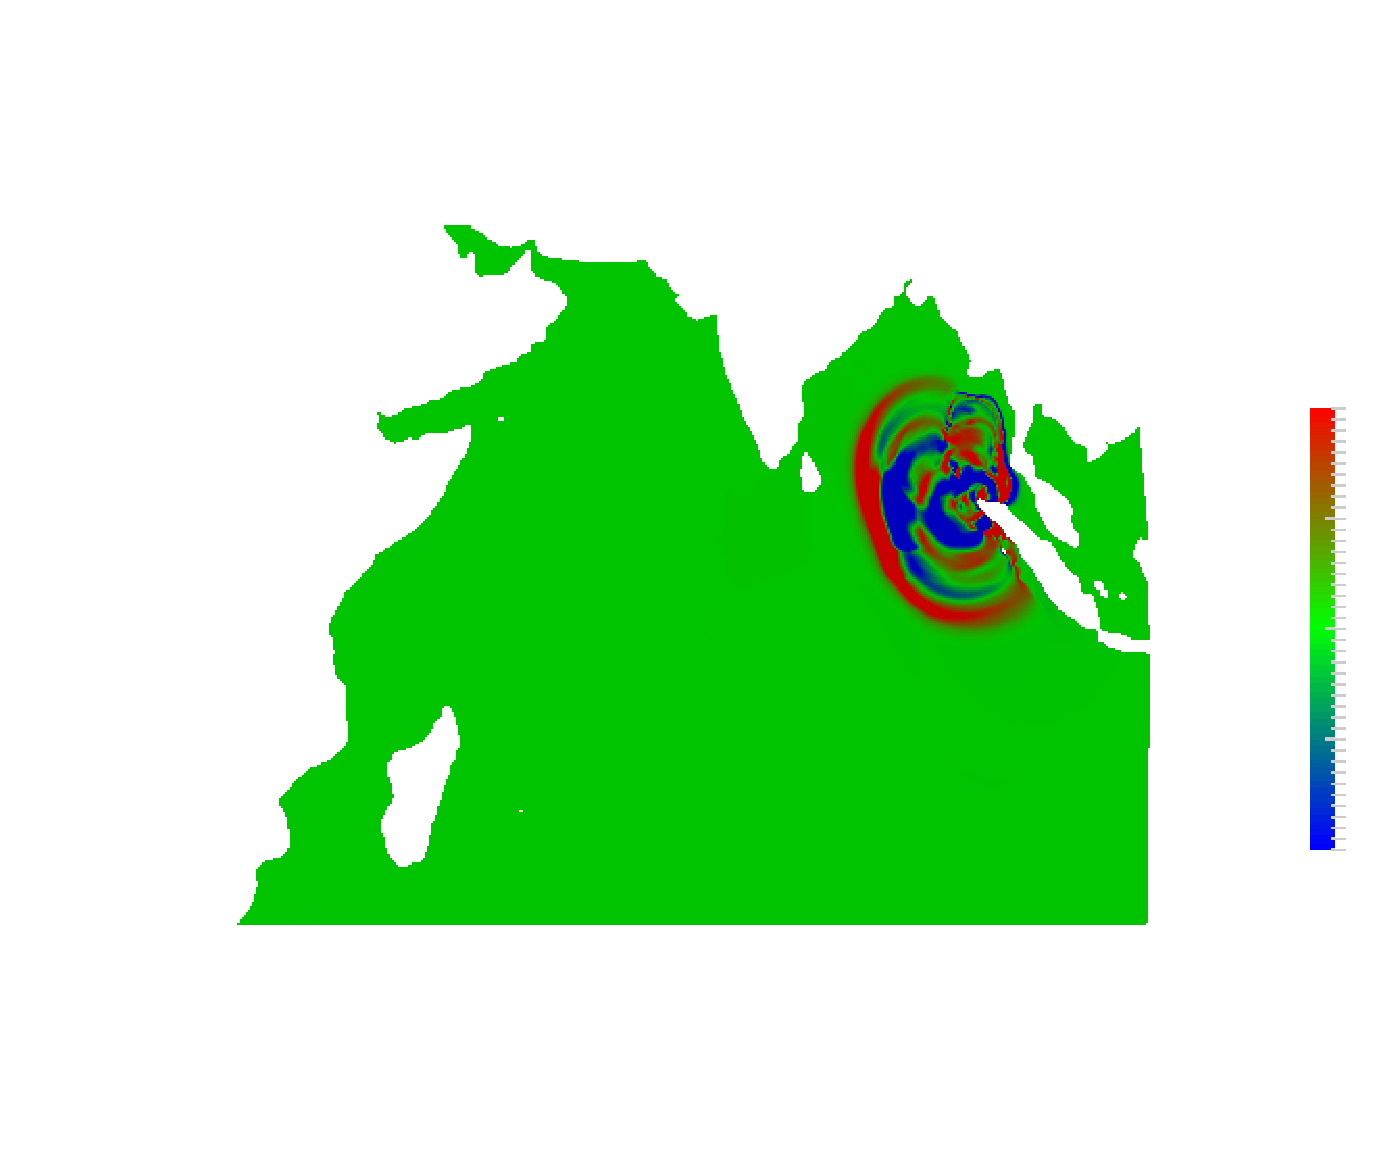
\includegraphics[trim=3.95cm 3.95cm 3.95cm 3.95cm,clip=true,width=\textwidth]{./figures/T80N4.pdf}
  \end{minipage}}\\
  \centering
   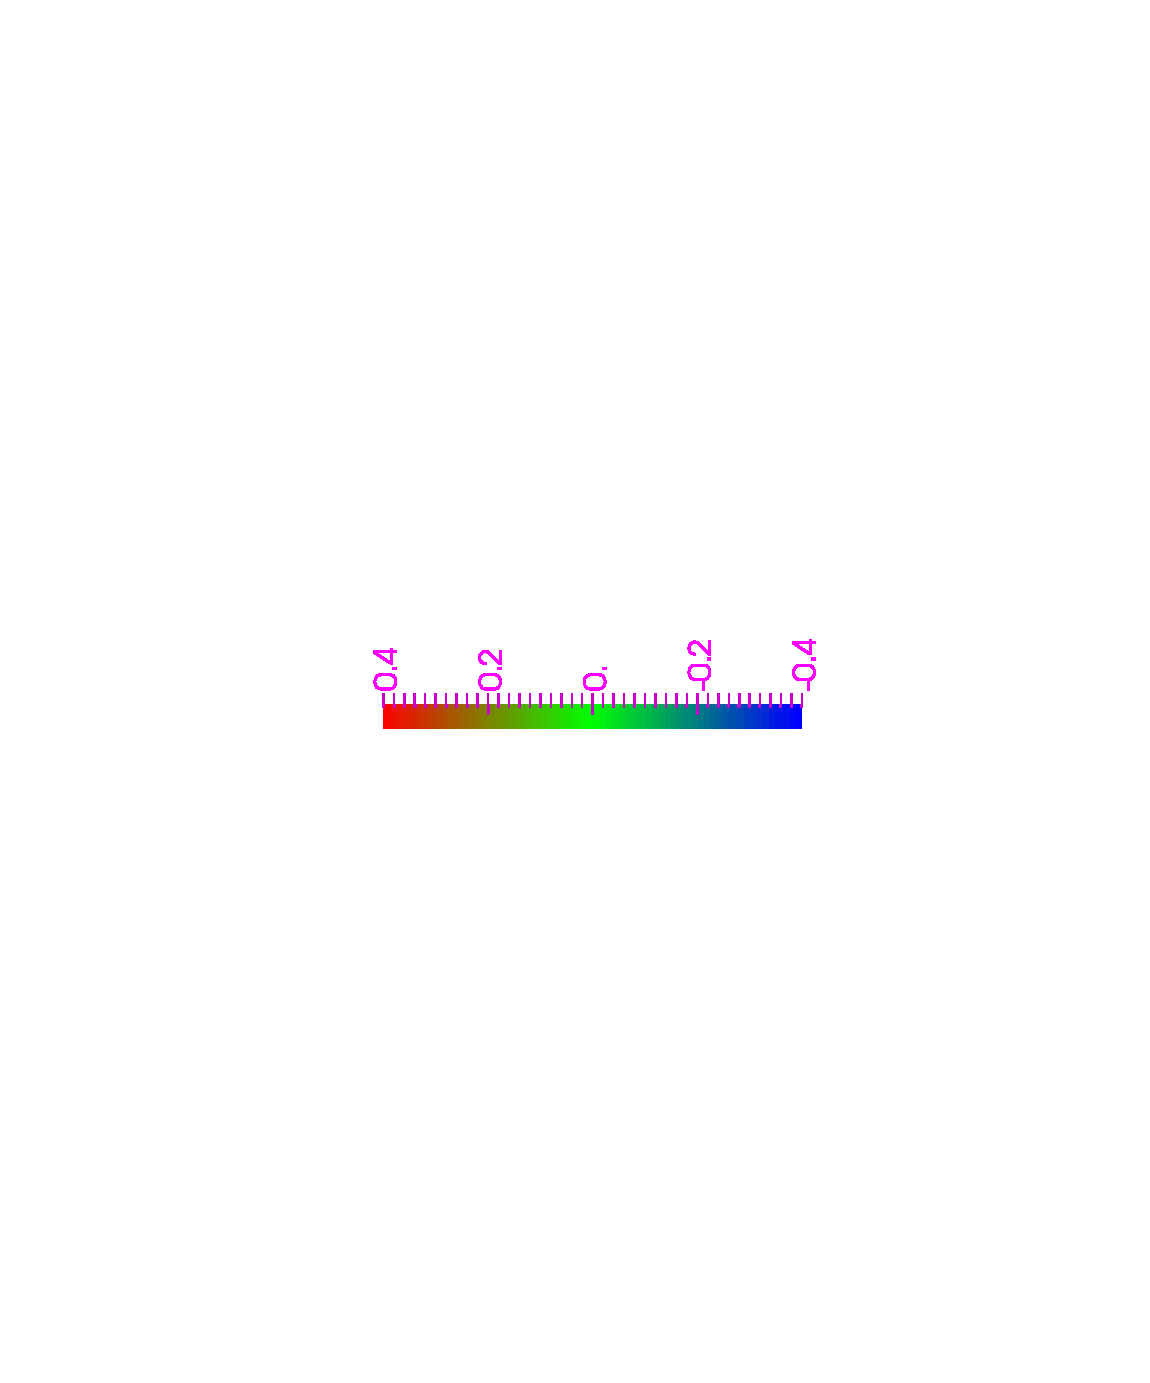
\includegraphics[trim=6cm 11cm 5cm 10.5cm,clip=true,width=0.5\textwidth]{./figures/TsunamiLegend.pdf}
\end{center}
 \caption{\emph{Free surface elevation of Indian Ocean tsunami at $80$ minutes
after earthquake. Simulations are run with $1$, $2$, $3$, and $4^{th}$ order
respectively.}}
  \label{fig:tsunami_propagation_compare_N}
\end{figure}


\subsection{Arrival time map}
One of the most important parameters in planning the evacuation in disaster management is the arrival time of the tsunamis. A surface plot of arrival time of the tsunami in the Indian Ocean and the coastal regions is shown in Fig (\ref{fig:arrivalTimeMap}). The arrival time is considered to be the time at which a free surface disturbance of $0.5m$ is observed for the first time. Using such arrival time maps, the critical regions can be identified during a real tsunami event. 
\begin{figure}[h!]
\begin{center}
%\centering
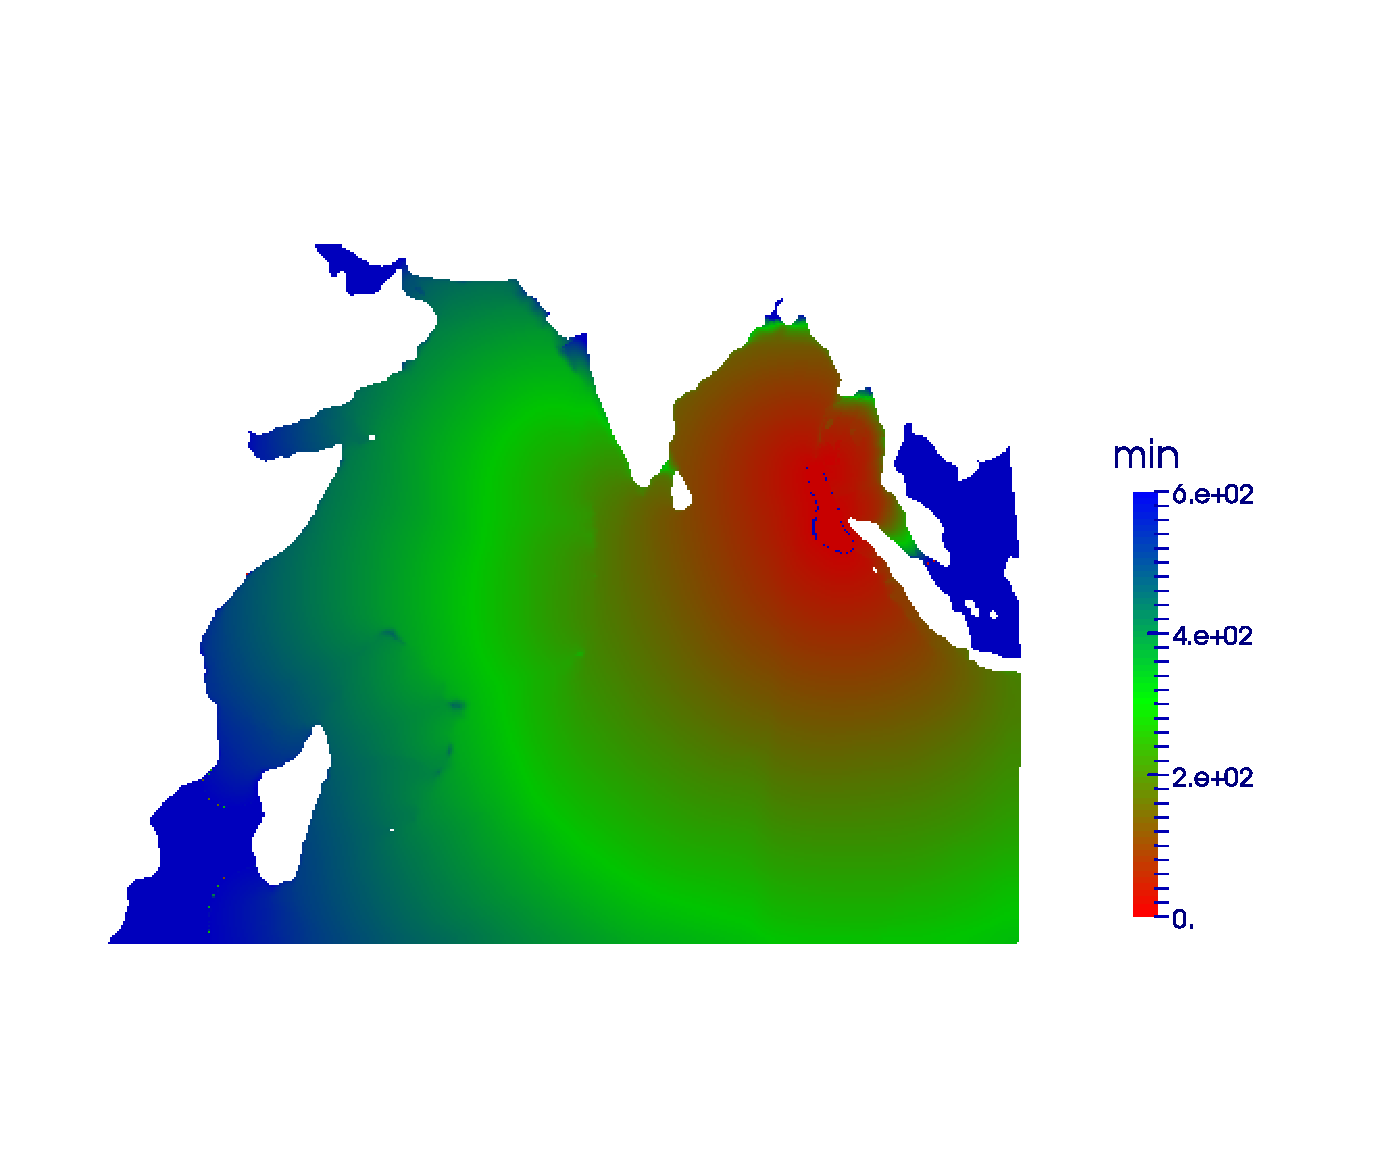
\includegraphics[trim=2cm 3cm 0cm 4cm,clip=true,width=0.5\linewidth]{./figures/arrivalTimeMapConN4.pdf}
\caption{\emph{Arrival time map in minutes. Simulations are ran using $4^{th}$ order polynomial representation in each triangle.}}
\label{fig:arrivalTimeMap}
\end{center}
\end{figure}

\subsection{Performance}
The performance of the kernels and efficiency of the overall solver with several threading models through the OCCA framework are presented in \cite{gandham2014swe} with the aid of analytical test cases. Here, the performance of the multi-rate scheme and overall solver for a realistic problem are presented. For the simulations, polynomial orders of $1$, $2$, $3$, and $4$ are considered.

Fig (\ref{fig:timeVsLevels}) shows the speedup achieved with multi-rate time stepping scheme with respect to the single rate scheme. The computational time required by the coarse elements decreases with the increase in number of levels. As a result, it is expected that the computational time decreases with the increasing number of levels used for the multi-rate scheme. However, the computations kernels are inefficient when the number of elements processed by the kernels is very low. Hence, there is no significant speedup when $4$ levels are used compared to when only $3$ levels are used for the simulation.  
\begin{figure}[h!]
\begin{center}
%\centering
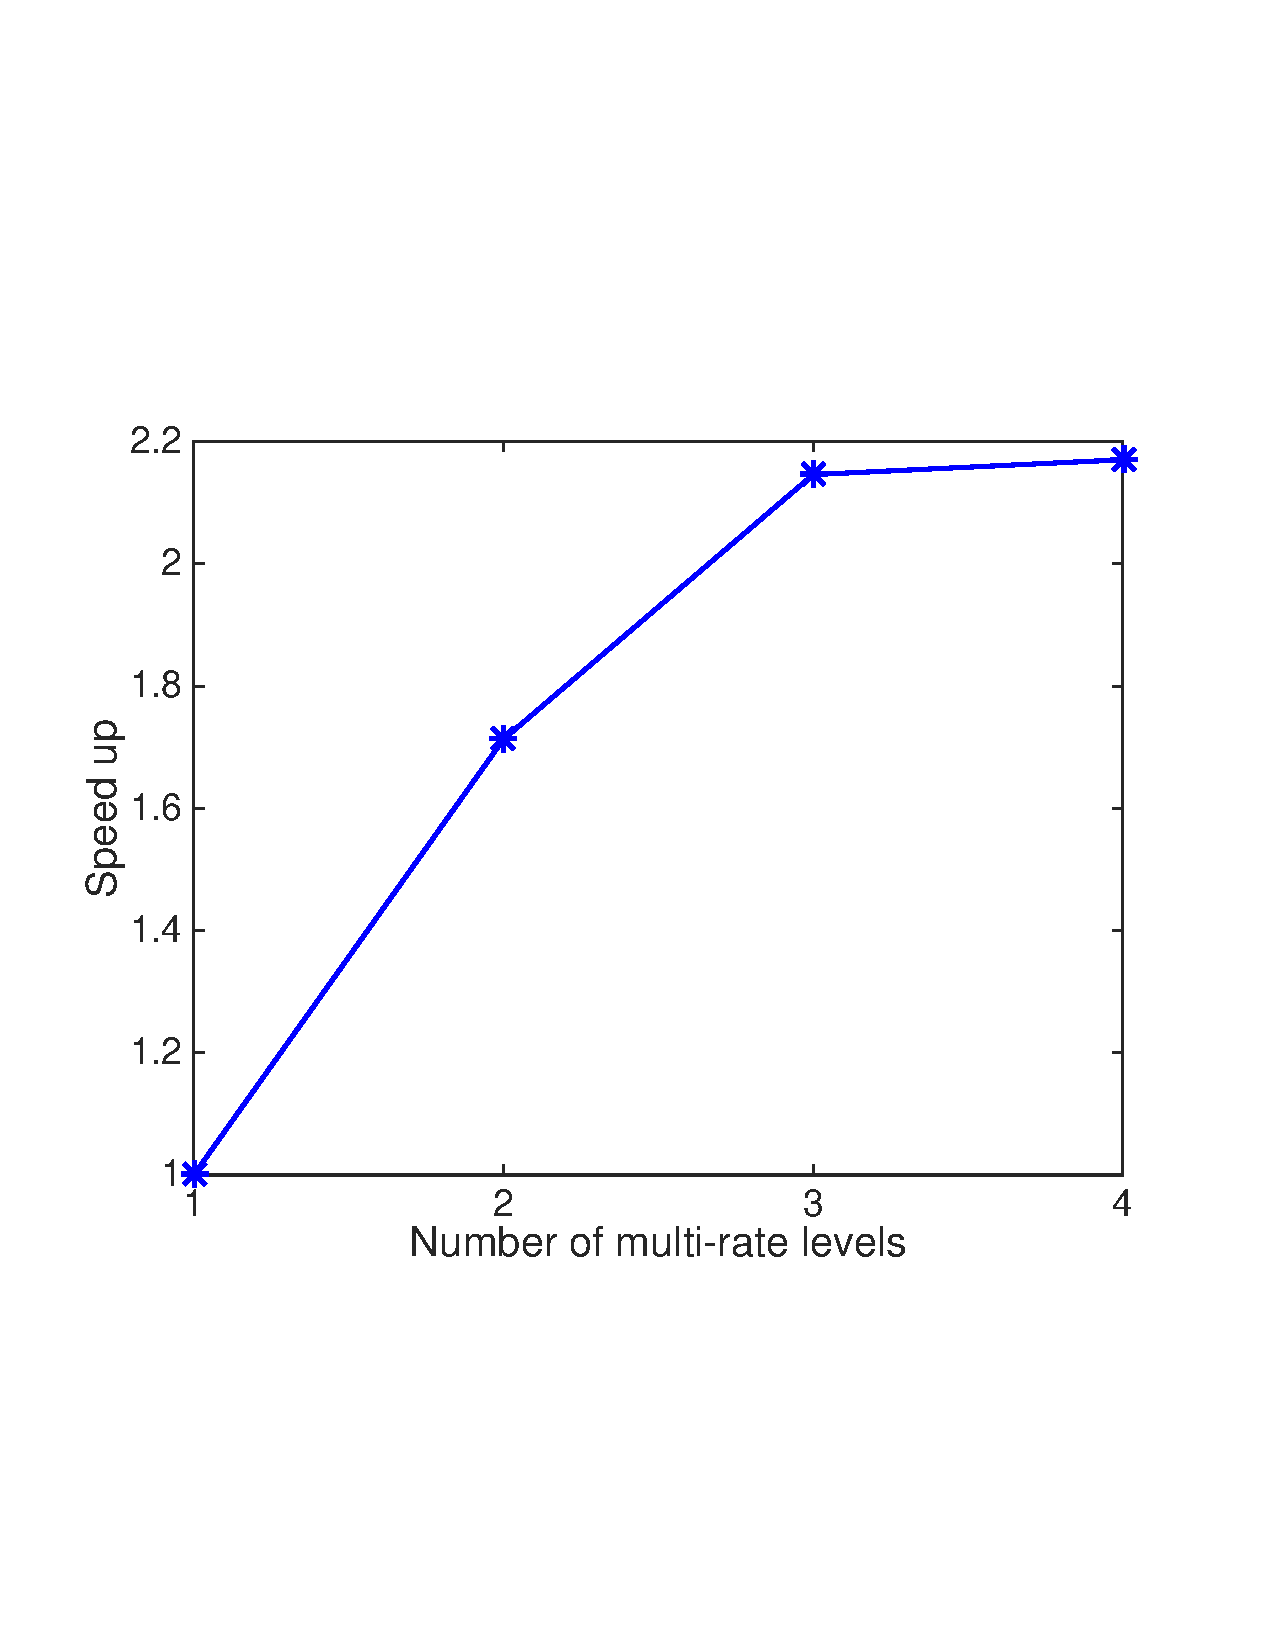
\includegraphics[trim=1cm 6cm 2cm 7cm,clip=true,width=0.5\linewidth]{./figures/timeVsLevels.pdf}
\caption{\emph{Overall speedup vs the number of multi-rate levels used for the simulation.}}
\label{fig:timeVsLevels}
\end{center}
\end{figure}

\begin{figure}[h!]
\begin{center}
%\centering
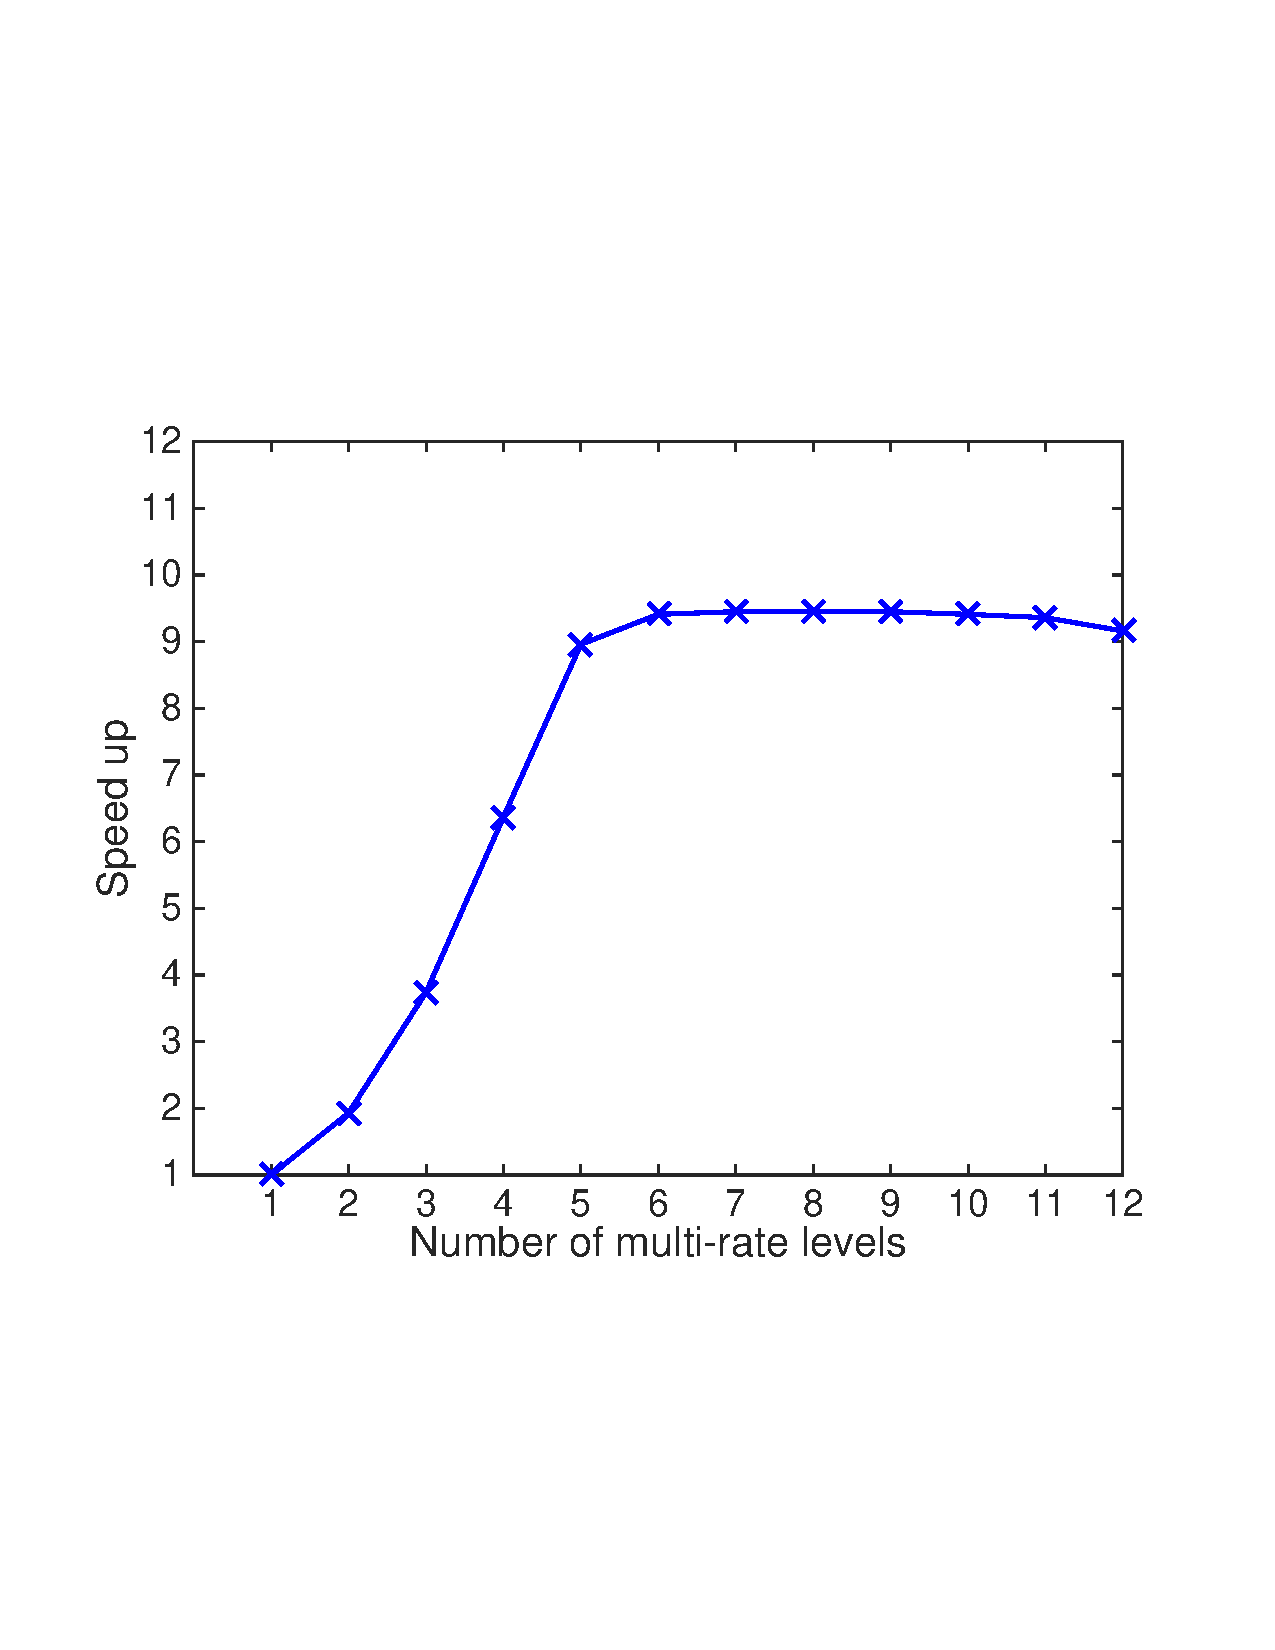
\includegraphics[trim=1cm 6cm 2cm 7cm,clip=true,width=0.5\linewidth]{./figures/timeVsLevelsWorldOcean.pdf}
\caption{\emph{Overall speedup vs the number of multi-rate levels used for
the simulation.}}
\label{fig:timeVsLevelsWorldOcean}
\end{center}
\end{figure}

%Fig (\ref{fig:profile_multirate}) illustrates the percentage of time spent on each level during the simulation. From the Table (\ref{tab:pasidgLevels}), the expected computational cost for $2\%$ of the elements correspond to the finest level is about $6\%$. However,  the computational time spent is more than $10\%$ of the overall time in all the cases. This is because of the under-utilization of the hardware when only fewer elements are processed by a computational kernel.
%\begin{figure}%[h!]
%\begin{center}
%  \subfloat[N=1]{%
%    \begin{minipage}[c]{0.2\linewidth}
%      \centering%
%      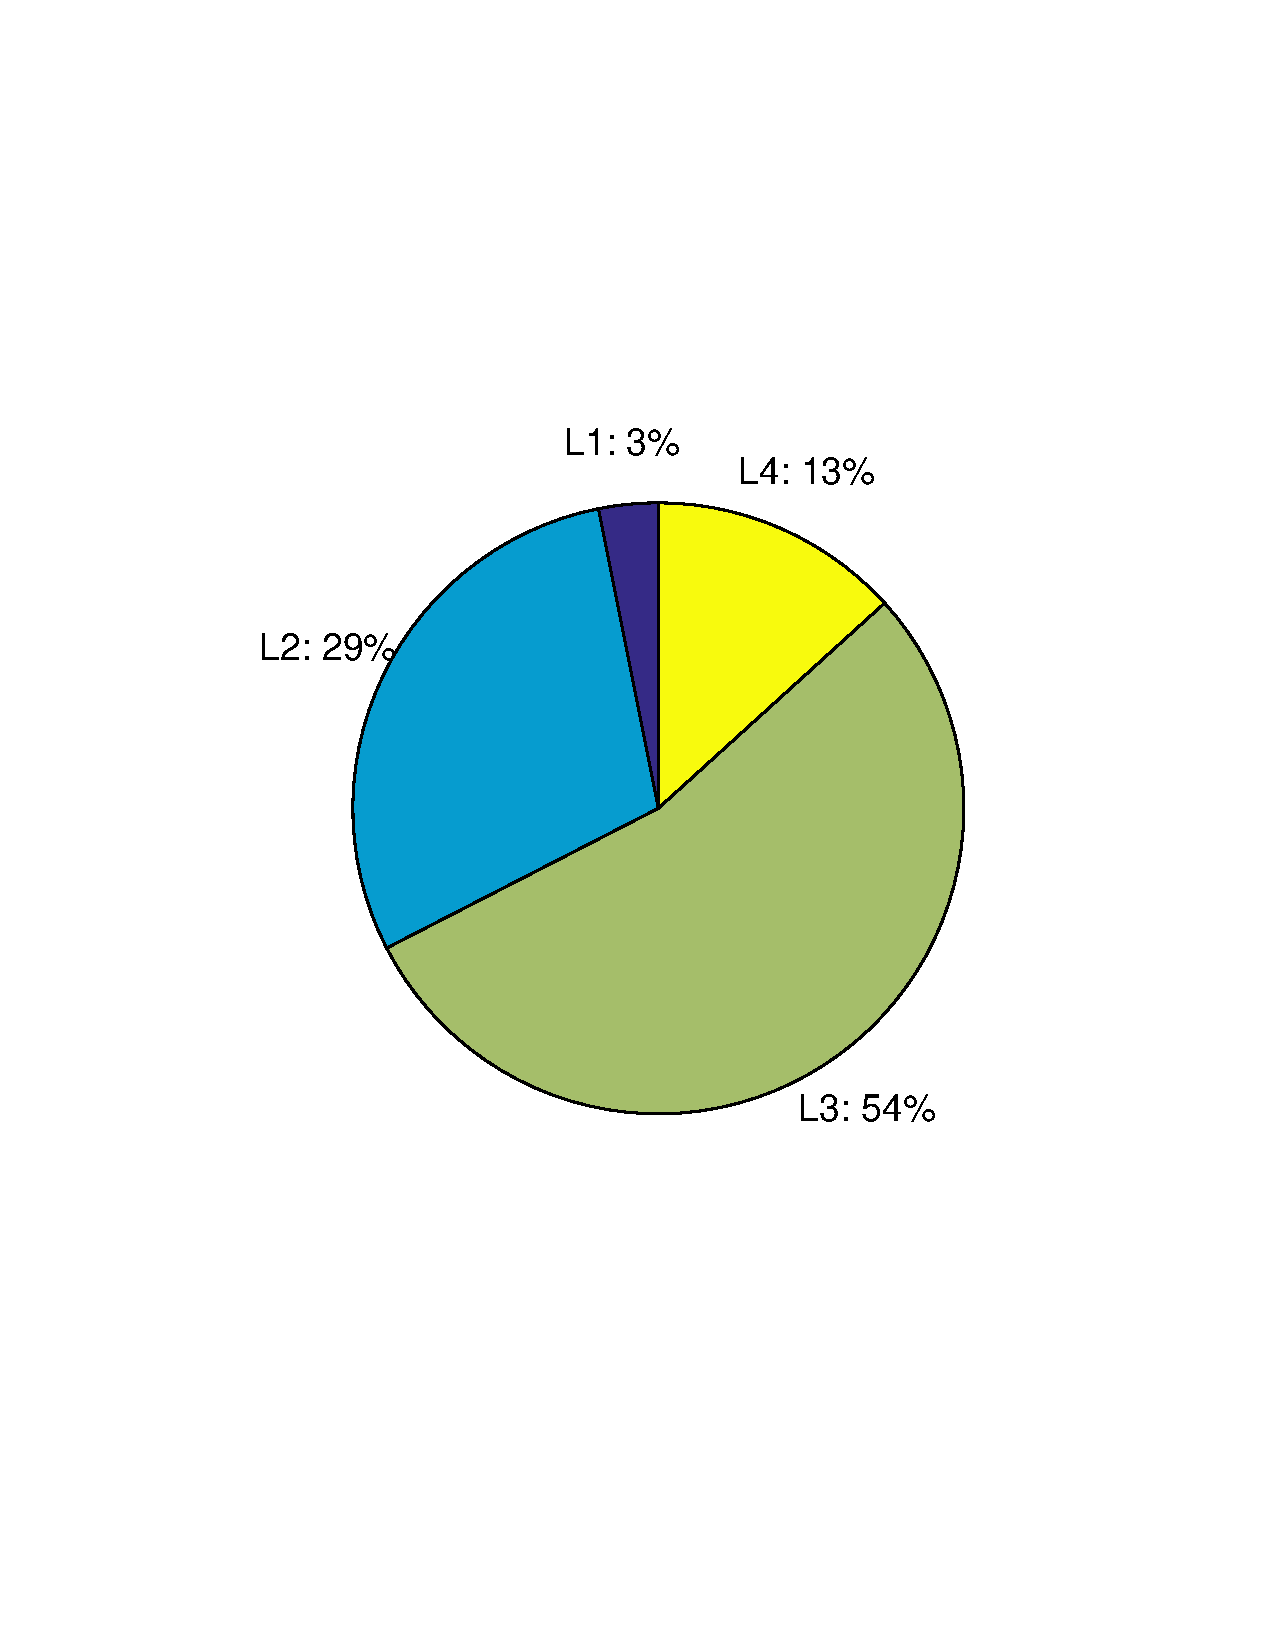
\includegraphics[trim=4cm 8.5cm 2cm 7cm,clip=true,width=\textwidth]{./figures/profileMultirateCudaN1.pdf}
%  \end{minipage}} \hspace{0.3cm}
%  \subfloat[N=2]{%
%    \begin{minipage}[c]{0.2\linewidth}
%      \centering%
%      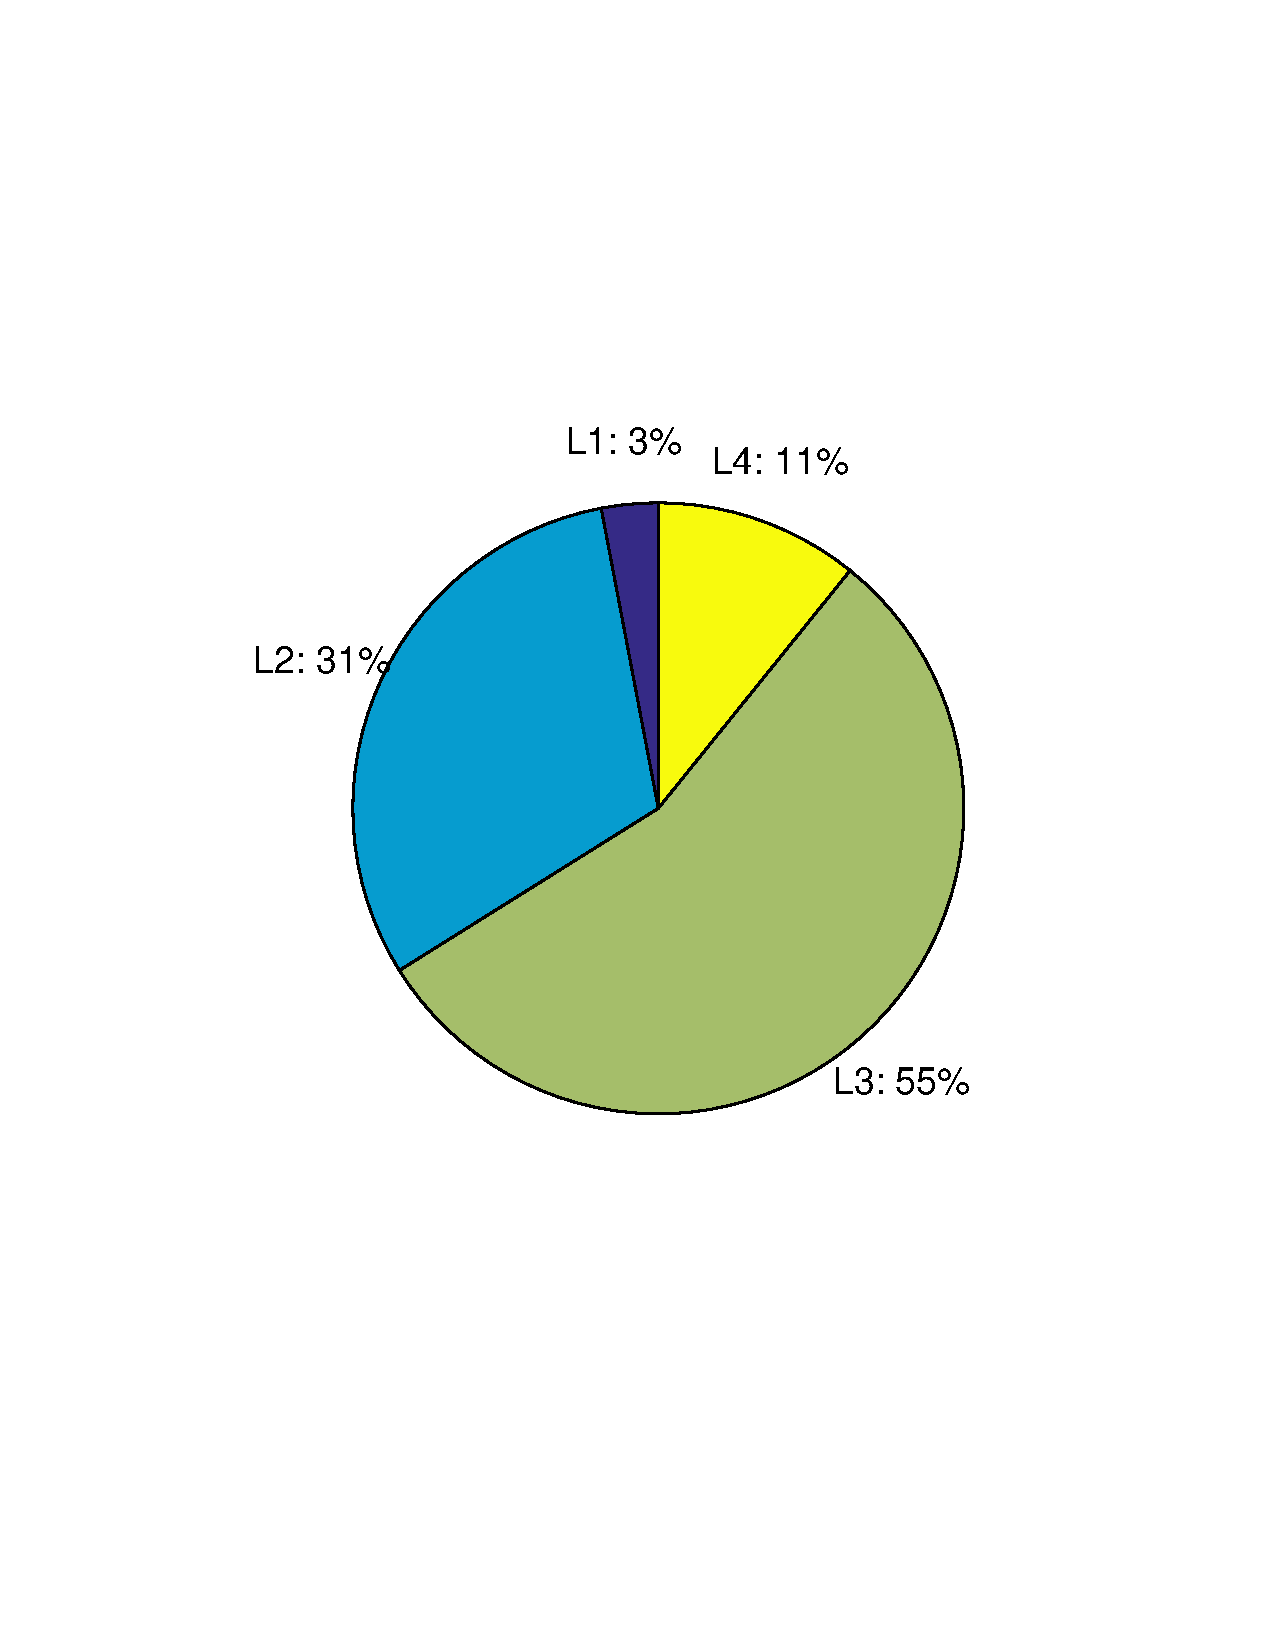
\includegraphics[trim=4cm 8.5cm 2cm 7cm,clip=true,width=\textwidth]{./figures/profileMultirateCudaN2.pdf}
%  \end{minipage}}\hspace{0.3cm}
%    \subfloat[N=3]{%
%    \begin{minipage}[c]{0.2\linewidth}
%      \centering%
 %     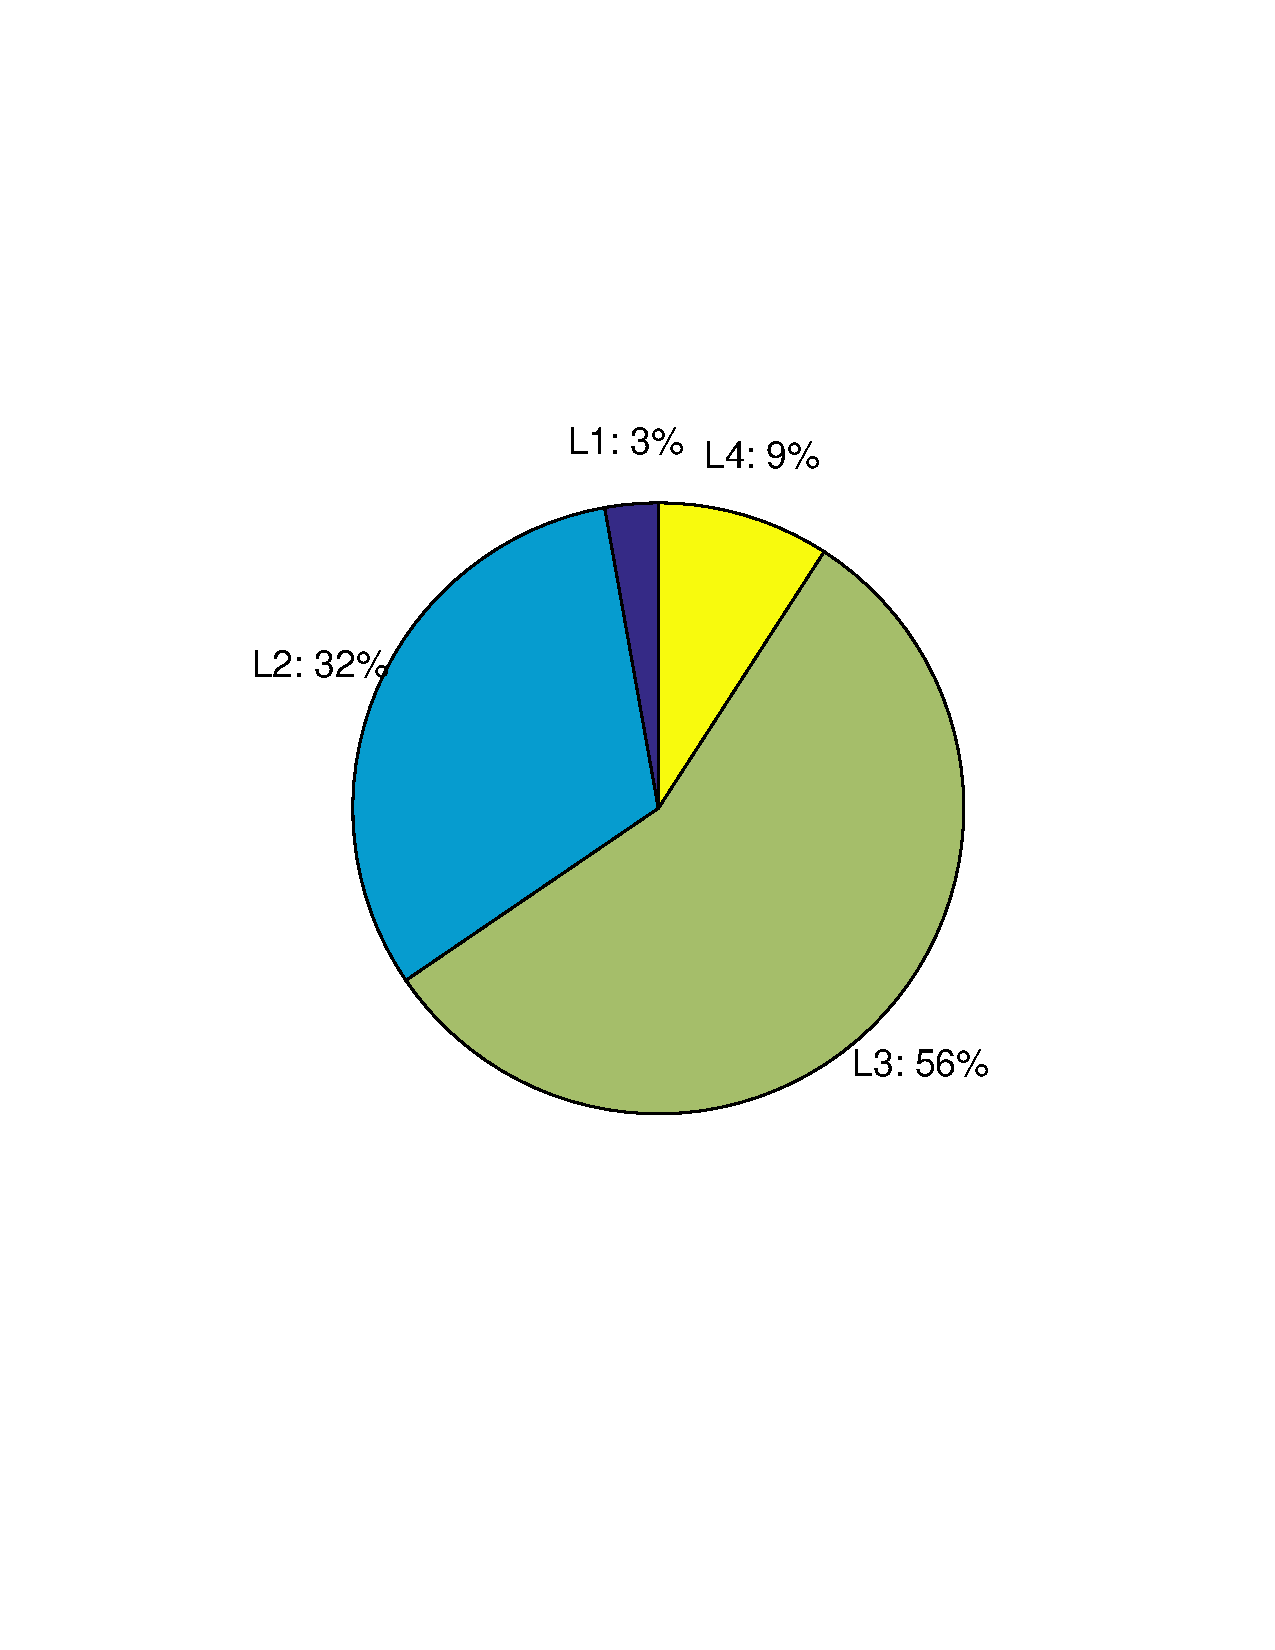
\includegraphics[trim=4cm 8.5cm 2cm 7cm,clip=true,width=\textwidth]{./figures/profileMultirateCudaN3.pdf}
 % \end{minipage}} \hspace{0.3cm}
%  \subfloat[N=4]{%
 %   \begin{minipage}[c]{0.2\linewidth}
 %     \centering%
 %     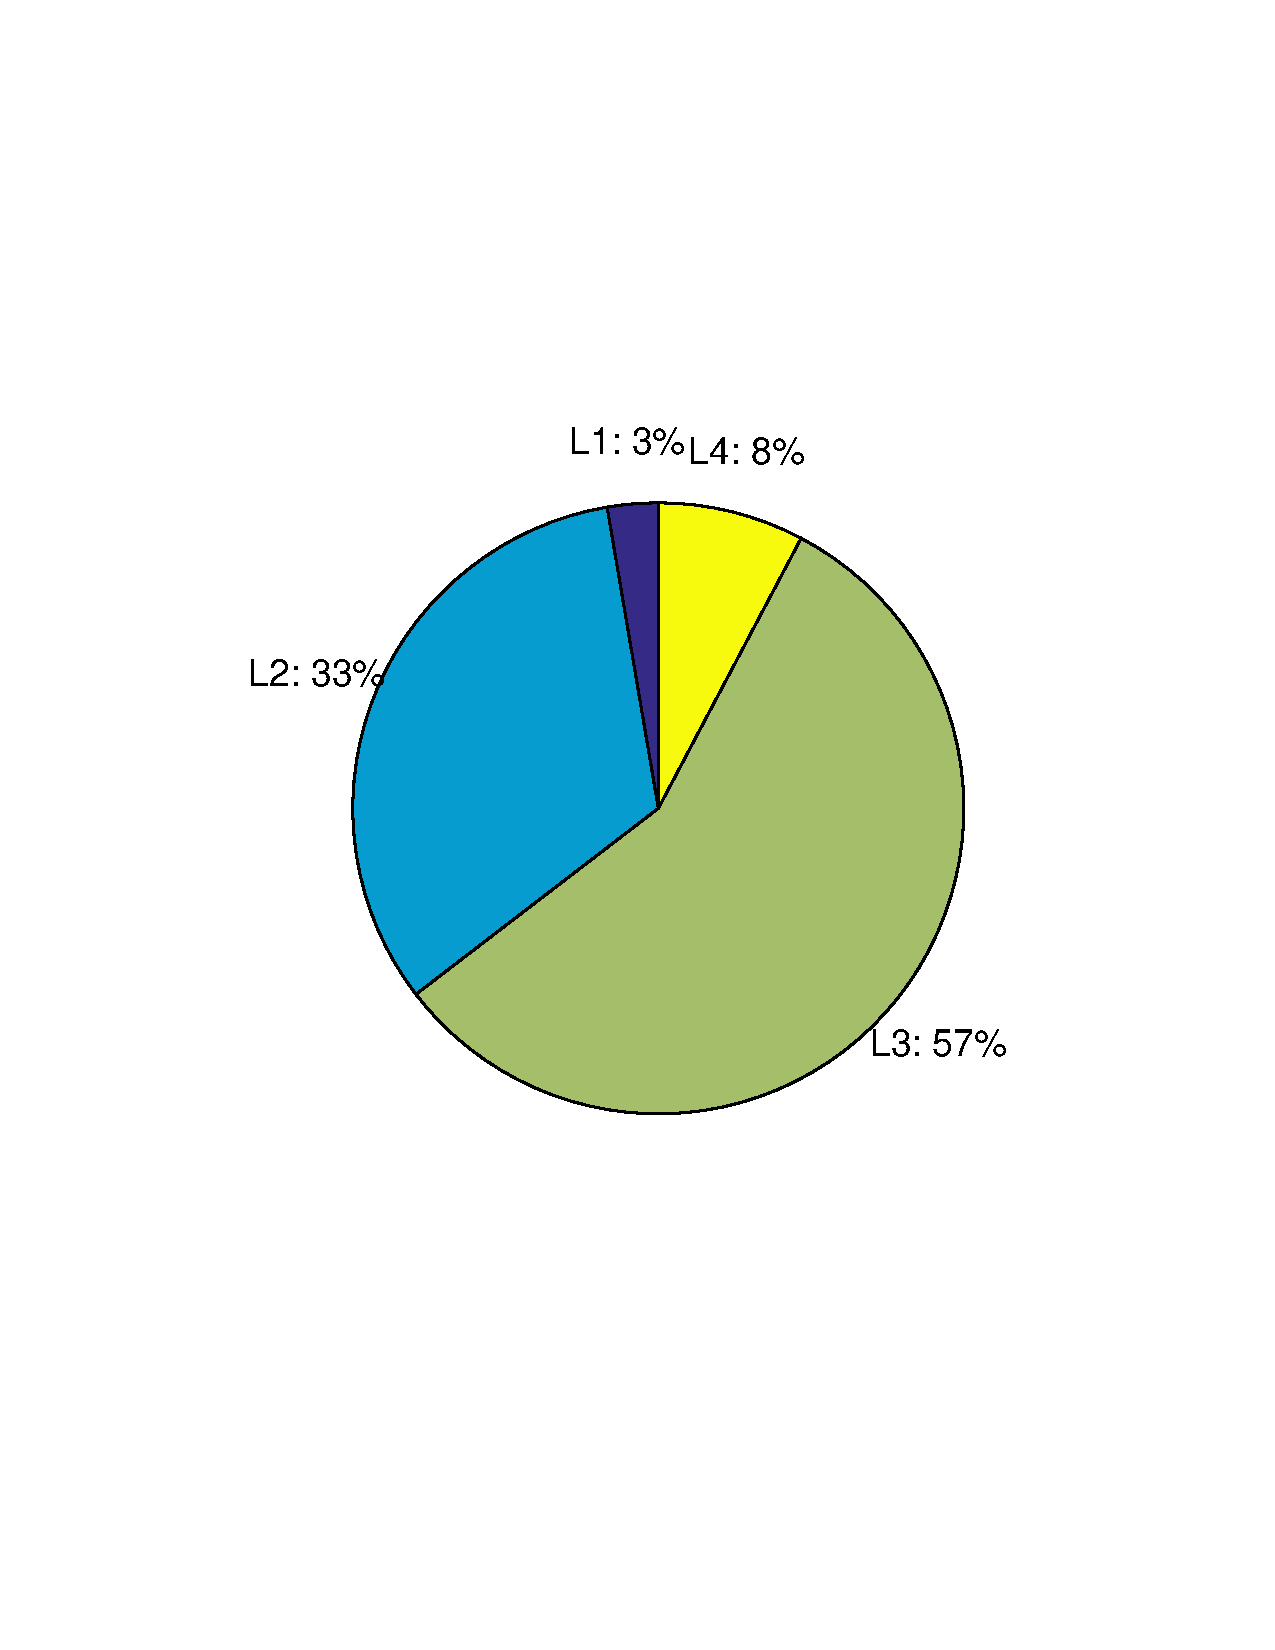
\includegraphics[trim=4cm 8.5cm 2cm 7cm,,clip=true,width=\textwidth]{./figures/profileMultirateCudaN4.pdf}
 % \end{minipage}}
%\end{center}
 %\caption{\emph{Percentage of time spent by each level in the multi-rate time scheme. Simulations are run on one NVIDIA K40c GPU.}}
 % \label{fig:profile_multirate}
%\end{figure}


 The overall computational time for the simulations using polynomial orders $1$, $2$, $3$, and $4$ are given in Tables (\ref{tab:pasidgTiming}, \ref{tab:worldOceanTiming}).  The kernels are tuned using parameters described in \cite{gandham2014swe}. Using CUDA model on NVIDIA K40c GPU, the simulations run as fast as $130$ times the faster than real time with linear polynomials while running at $10$ times faster with $4^{th}$ order polynomials in each triangle, in case of Indian Ocean tsunami.
In these experiments, a single mesh is used for all the discretizations. However, a coarser mesh may provide similar predictions for higher order DG discretizations.
\begin{table}[h!]
\begin{center}
\begin{tabular}{crrr}
\hline
Polynomial & \# unknowns & Compute& Real/  \\
order & (millions)& time (min) & compute\\ \hline
1 & 1.17 &  5 & 130\\
2 & 2.34 & 14 &  41\\
3 & 3.90 & 33 &  18\\
4 & 5.85 & 64 &  10\\\hline
\end{tabular}
\caption{\emph{The overall compute time of 10 hrs of Indian Ocean tsunami simulation using an NVIDIA K40c GPU. The simulation used OCCA:CUDA model and single precision arithmetic.}}
\label{tab:pasidgTiming}
\end{center}
\end{table}

\begin{table}[h!]
\begin{center}
\begin{tabular}{crrr}
\hline
Polynomial & \# unknowns & Compute& Real/  \\
order & (millions)& time (min) & compute\\ \hline
1 & 15.8 &  36 & 16\\
2 & 31.6 & 100 &  6\\
3 & 52.7 & 220 & 2.7\\
4 & 79.1 & 460 & 1.3\\\hline
\end{tabular}
\caption{\emph{The overall compute time of 10 hrs of Japan tsunami
simulation using an NVIDIA K40c GPU. The simulation used OCCA:CUDA model
and single precision arithmetic.}}
\label{tab:worldOceanTiming}
\end{center}
\end{table}
%\section{Results: 2011 Japan tsunami}
%\subsection{Performance}

%ADD timing results for OpenCL, OpenMP.






%% conclusions
%% future work (wetting and drying if its not included already, full 3D models instead of Boussinesq models)

\section{Conclusions}
We demonstrated the efficiency of a GPU accelerated discontinuous Galerkin method for real world tsunami simulations. The performance results indicate that faster than real-time tsunami simulations are possible even with high order discretizations on a workstation.  The reasons contributing to such performance are: 
\begin{enumerate}
\item Tailoring the implementations specifically for the discontinuous Galerkin discretization of shallow water equations gives significantly increased performance compared to a more general library-based approach.
\item An order of magnitude performance improvement is achieved by taking advantage of GPUs. This required exposing fine-grain parallelism in the algorithms. \item Multi-rate time stepping method improves the time stepping performance by allowing the elements to be integrated with local allowable time step sizes. The speed up with the multi-rate scheme is ten folds for global tsunami simulation. 
\item Using single precision arithmetic gives up to  two fold speed up compared to double precision arithmetic on GPUs since the algorithms are memory bound.  
\end{enumerate}
\section*{Acknowledgements}
The authors gratefully acknowledge travel grants from Pan-American Advanced Studies Institute,  grant from DOE and ANL (ANL Subcontract No. 1F-32301 on DOE grant No. DE-AC02-06CH11357),  grant from ONR (Award No. N00014-13-1-0873),  fellowships from Ken Kennedy Institute of technology at Rice University and support from Shell (Shell Agreement No. PT22584), NVIDIA, and AMD.  Authors also thank  Axel Modave, Jesse Chan, and Bruno Seny for fruitful discussions in preparation of this manuscript.


\bibliographystyle{siam}
\bibliography{refs}
\end{document}
